\documentclass[12pt]{report}
\usepackage{babel}
\usepackage[utf8]{inputenc}
\usepackage[T1]{fontenc}
\usepackage{vntex}
\renewcommand{\baselinestretch}{1.2} 
\PassOptionsToPackage{table}{xcolor}
\usepackage[table]{xcolor}
%\usepackage[utf8]{inputenc}
%\usepackage[francais]{babel}
%\usepackage[margin=0.5in]{geometry}
\usepackage{geometry}
\usepackage{a4wide,amssymb,epsfig,latexsym,multicol,array,hhline}
\usepackage{lastpage}
\usepackage{emptypage}
\usepackage{pdfpages}
\usepackage[lined,boxed,commentsnumbered]{algorithm2e}
\usepackage{enumerate}
\usepackage{color}
\usepackage{spverbatim}
\usepackage{graphicx}							% Standard graphics package
\usepackage{array}
\usepackage{tabularx}
\usepackage{multirow}
\usepackage{multicol}
\usepackage{rotating}
\usepackage{graphics}
\usepackage[labelsep=endash]{caption}

% keep figure in subsection
\usepackage[section]{placeins} 
\usepackage{flafter}

\usepackage{setspace}
\usepackage{epsfig}
\usepackage{tikz}
\usetikzlibrary{arrows,snakes,backgrounds}
\usepackage{hyperref}
% check reference if not cite
%\usepackage{refcheck}
\usepackage{cleveref}
\hypersetup{urlcolor=blue,linkcolor=black,citecolor=black,colorlinks=true} 
\usepackage{shapepar}
\usepackage{titlesec}
\usepackage{mdframed}
\usepackage{mathtools}
\usepackage{amsmath}
\usepackage{amssymb}
\usepackage{changepage}
% pseudocode
\usepackage[lined,boxed,commentsnumbered]{algorithm2e}
\usepackage{tabularx, caption}
\usepackage{qtree}
\usepackage{pgfgantt}
\usepackage{pgfplots}
\usepackage{tkz-euclide}
\usepackage{accents}
\usepackage{setspace}
\usepackage{animate}
\usepackage{lipsum}
\usepackage{verbatim}

\usetikzlibrary{arrows,snakes,backgrounds,automata,positioning,trees,shapes,calc,through,bending}
\usetikzlibrary{datavisualization}
\usetikzlibrary{datavisualization.formats.functions}
\usepackage{movie15}
\usepackage{pst-plot}
\usepackage[numbered]{bookmark}
\usepackage{tocloft}
\usepackage{helvet}
\usepackage{listings}
\usepackage[ddmmyyyy]{datetime}
\usepackage{csvsimple}
\usepackage{float}
\usepackage{cases}
%\usepackage[nomessages]{fp}
\usetkzobj{all} 
%\usepackage{pstcol} 								% PSTricks with the standard color package

%\usepackage[backend=bibtex,style=authoryear,natbib=true]{biblatex}
%\usepackage[autostyle=true]{csquotes}
%,citestyle=numeric
\usepackage[backend=bibtex]{biblatex} % Use the bibtex backend with the authoryear citation style (which resembles APA)

\addbibresource{bibliography.bib}

%\usepackage[autostyle=true]{csquotes} % Required to generate language-dependent quotes in the bibliography

\newtheorem{theorem}{{\bf Định lý}}
\newtheorem{constraint}{{\bf Ràng buộc}}
\newtheorem{property}{{\bf Tính chất}}
\newtheorem{proposition}{{\bf Mệnh đề}}
\newtheorem{corollary}[proposition]{{\bf Hệ quả}}
\newtheorem{lemma}[proposition]{{\bf Bổ đề}}


%%ensembles de nombres
\def\NP{$\mathcal{NP}$}
\def\N{\mathbb{N}}
\def\Z{\mathbb{Z}}
\def\R{\mathbb{R}}
\def\Q{\mathbb{Q}}
\addto\captionsenglish{% Replace "english" with the language you use
  \renewcommand{\contentsname}{Mục lục}
  \renewcommand{\listfigurename}{Danh mục hình ảnh}
  \renewcommand{\chaptername}{Chương}
  \renewcommand{\figurename}{Hình}
  \renewcommand{\abstractname}{Tóm tắt}
  \renewcommand{\bibname}{Tài liệu tham khảo}  
  \renewcommand{\refname}{Tài liệu tham khảo}  
  %
}
\newcolumntype{M}[1]{>{\centering\arraybackslash}m{#1}}
\newcolumntype{P}[1]{>{\centering\arraybackslash}p{#1}}
%\def\myd#1{\text{\d{\ensuremath#1}}}


\newcounter{numproblem}
\newenvironment{problem}{\addtocounter{numproblem}{1}
\noindent{\large \bf Problem \thenumproblem. }}{}

\newcounter{numexercise}
\newenvironment{exercise}{\addtocounter{numexercise}{1}
\noindent{\large \bf Exercise \thenumexercise. \\}}{}

\newcounter{numquestion}
\newenvironment{question}{\addtocounter{numquestion}{1}
\noindent{\large \bf Question \thenumquestion. \\}}{}


\newcounter{numcau}
\newenvironment{cau}{\addtocounter{numcau}{1}
\noindent{\large \bf Câu \thenumcau. \\}}{}

%\newcounter{numsolution}
\newenvironment{solution}{
\noindent{ \large \bf Solution.\\}  \color{blue}}{~~\hfill$\Box$\\}

\newenvironment{loigiai}{
\noindent{ \large \bf Lời giải.\\}  \color{blue}}{~~\hfill$\Box$\\}

\newif\ifshortversion
\shortversiontrue 	% hide this line when shortversion==false
\newcommand\version[2]{\ifshortversion #1 \else #2 \fi}

\newcommand{\tikzAngleOfLine}{\tikz@AngleOfLine}
\def\tikz@AngleOfLine(#1)(#2)#3{%
\pgfmathanglebetweenpoints{%
\pgfpointanchor{#1}{center}}{%
\pgfpointanchor{#2}{center}}
\pgfmathsetmacro{#3}{\pgfmathresult}%
} 


%\usepackage{fancyhdr}
\definecolor{darkblue}{RGB}{3, 43, 145}
\definecolor{lightblue}{RGB}{20, 136, 219}
\definecolor{amber}{rgb}{1.0, 0.75, 0.0}
\definecolor{aqua}{rgb}{0.0, 1.0, 1.0}
\definecolor{dkgreen}{rgb}{0,0.6,0}
\definecolor{gray}{rgb}{0.5,0.5,0.5}
\definecolor{mauve}{rgb}{0.58,0,0.82}
\definecolor{awesome}{rgb}{1.0, 0.13, 0.32}
\definecolor{banana}{rgb}{1.0, 0.88, 0.21}
\definecolor{brilliantlavender}{rgb}{0.96, 0.73, 1.0}
\definecolor{bubbles}{rgb}{0.91, 1.0, 1.0}
\newsavebox\LogoHCMUT
\savebox\LogoHCMUT{%
\centering
\renewcommand{\familydefault}{\sfdefault}
\normalfont
\begin{tikzpicture}[shorten >=1pt,node distance=1.5cm,on grid,auto,/tikz/initial text=,font=\small,align=center] 
 \newdimen\R
 \newdimen\fsbk
 \newdimen\fshcm
   \R=142pt
   \fsbk=135pt
   \fshcm=50pt
   \coordinate (O) at (0:0) {};
   \node (BK) at ($(0:0)+(90:\R/7)$)[draw=none] {\color{darkblue} \bf 
   \begingroup
    \fontsize{\fsbk}{\fsbk}\selectfont
     BK
	\endgroup
	\\};
   \node  (HCM) at ($(BK.south)+(-90:\R/7)$)[draw=none] {\color{lightblue} \bf 
   \begingroup
    \fontsize{\fshcm}{\fshcm}\selectfont
    \centering
    \hspace{-1pt} TP.HCM
	\endgroup
	\\};
   \foreach \x in {0,60,...,360}  {\draw[draw = none] ($(O)+(\x+30:\R)$) -- ($(O)+(\x+90:\R)$);}
   \foreach \i in {0,120,240} {
    \draw[fill=darkblue,draw = none] ($(O)+(\i+150:\R)$) -- ($(O)+(\i+150:\R)+(\i+90:\R)$) -- ($(O)+(\i+90:\R)+(\i+90:\R)$) -- ($(O)+(\i+90:\R)$) -- cycle;
   \draw[fill=lightblue,draw = none] ($(O)+(\i+30:\R)$) -- ($(O)+(\i+30:\R)+(\i+90:\R)$) -- ($(O)+(\i+90:\R)+(\i+90:\R)$) -- ($(O)+(\i+90:\R)$) -- cycle;
   }
\end{tikzpicture}
\renewcommand{\familydefault}{\rmdefault}
\normalfont
}
\newcommand{\insertlogo}[2]{\resizebox{#1}{#2}{\usebox{\LogoHCMUT}}}%



\newbox\one
\newbox\two
\long\def\loremlines#1{%
    \setbox\one=\vbox {%
      \lipsum
     }
   \setbox\two=\vsplit\one to #1\baselineskip
   \unvbox\two}
   
   \setcounter{secnumdepth}{4}
\setcounter{tocdepth}{3}
\makeatletter
\newcounter {subsubsubsection}[subsubsection]
\renewcommand\thesubsubsubsection{\thesubsubsection .\@alph\c@subsubsubsection}
\newcommand\subsubsubsection{\@startsection{subsubsubsection}{4}{\z@}%
                                     {-3.25ex\@plus -1ex \@minus -.2ex}%
                                     {1.5ex \@plus .2ex}%
                                     {\normalfont\normalsize\bfseries}}
\newcommand*\l@subsubsubsection{\@dottedtocline{3}{10.0em}{4.1em}}
\newcommand*{\subsubsubsectionmark}[1]{}

%%% mathematic
\newcommand\givenbase[1][]{\:#1\lvert\:}
\let\given\givenbase
\newcommand\sgiven{\givenbase[\delimsize]}
\DeclareMathOperator*{\argmin}{argmin}
\DeclareMathOperator*{\argmax}{argmax}

% numbering eq iff ref
\mathtoolsset{showonlyrefs=true}
%\DeclarePairedDelimiterX\Basics[1](){\let\given\sgiven #1}
%\newcommand\Average{E\Basics}

%%%%%%%%%%%%%%%%%%%%%%%%%%%%%%%%%%%%%%%%%%%
% Dkl
\DeclarePairedDelimiterX{\infdivx}[2]{(}{)}{%
	#1\;\delimsize\|\;#2%
}
\newcommand{\Dkl}{D_{KL}\infdivx}
\DeclarePairedDelimiter{\norm}{\lVert}{\rVert}


%%%%%%%%%%%%%%%%%%%%%%%%%%%%%%%%%%%%%%%%%%%

\makeatother


%%%%%%%%%%%%%%%%%%%%%%%%%%%%%%%%%%%%%%


%\newcommand{\tikzAngleOfLine}{\tikz@AngleOfLine}
\def\tikz@AngleOfLine(#1)(#2)#3{%
\pgfmathanglebetweenpoints{%
\pgfpointanchor{#1}{center}}{%
\pgfpointanchor{#2}{center}}
\pgfmathsetmacro{#3}{\pgfmathresult}%
} 

\def\roundloop[#1]#2#3{%
 \coordinate (rla) at (#2.east); 
 \path   (#2)--++(#1) coordinate (rlb);
 \tkzTgtFromP(#2,rla)(rlb)            
 \node (rlb) at (rlb) [circle through={(tkzFirstPointResult)}] {};
 \coordinate  (rlc) at (intersection 2 of #2 and rlb);
 \coordinate  (rld) at (intersection 1 of #2 and rlb);         
 \tikzAngleOfLine(rlb)(rld){\AngleStart}
 \tikzAngleOfLine(rlb)(rlc){\AngleEnd} 
 \tikzAngleOfLine(#2)(rlb){\AngleLabel}
 \ifdim\AngleStart pt<\AngleEnd pt
 \draw[thick,->]%
   let \p1 = ($ (rlb) - (rld) $), \n2 = {veclen(\x1,\y1)}
   in   
     (rlb) ++(\AngleLabel:\n2) node[]{#3}
     (rld) arc (\AngleStart:\AngleEnd:\n2); 
 \else 
  \draw[thick,->]%
   let \p1 = ($ (rlb) - (rld) $), \n2 = {veclen(\x1,\y1)}
   in   
     (rlb) ++(\AngleLabel:\n2) node[]{#3}
     (rld) arc (\AngleStart-360:\AngleEnd:\n2); 
   \fi 
  }
  
\graphicspath{{figures/}}

\newcommand{\executeiffilenewer}[3]{%
	\ifnum\pdfstrcmp{\pdffilemoddate{#1}}%
	{\pdffilemoddate{#2}}>0%
	{\immediate\write18{#3}}\fi%
}


\newcommand{\includesvg}[1]{%
	\executeiffilenewer{#1.svg}{#1.pdf}%
	{inkscape -z -D  --file=#1.svg --export-pdf=#1.pdf --export-latex}%
	\input{#1.pdf_tex}%
}


\title{Xây dựng mô hình dự đoán xu hướng\\ giá ngắn hạn các đồng tiền mật mã\\ bằng kĩ thuật học máy}								% Title								% Author
\date{\today}											% Date

\makeatletter
\let\thetitle\@title
\let\thedate\@date
\makeatother
\usepackage{tabularx}
\usepackage{tabularx,ragged2e}
\newcolumntype{C}{>{\Centering\arraybackslash}X}
\newcolumntype{L}{>{\arraybackslash}X}
\usepackage{fancyhdr}
\usepackage{float}
\usepackage{nameref}
\pagestyle{fancy}
\fancyhf{}
\fancyhead[RE]{\leftmark}
\fancyhead[LO]{\rightmark}
\fancyfoot[RO,LE]{\thepage}
\fancypagestyle{plain}{%  the preset of fancyhdr 
    \fancyhf{} % clear all header and footer fields
    \fancyfoot[C]{\textbf{\thepage}} % except the center
    \renewcommand{\headrulewidth}{0pt}
    \renewcommand{\footrulewidth}{0pt}}
    

\renewcommand\appendixpagename{Phụ lục}
\renewcommand\appendixtocname{Phụ lục}
%\renewcommand\algorithmautorefname{Thuật toán}
\renewcommand\algorithmcfname{Thuật toán}
%\newtheorem{algorithm}{}

\setcounter{secnumdepth}{4}

\usetikzlibrary{shapes,arrows}

\begin{document}

%\leavevmode\thispagestyle{empty}\newpage
%{leftmargin}{topmargin}{rightmargin}{bottommargin}{headheight}{headsep}{footheight}{footskip}
\setmarginsrb{3.0 cm}{-1.0 cm}{2.0 cm}{2.0 cm}{1.2 cm}{1 cm}{1.2 cm}{1 cm}
\begin{titlepage}
\begin{center}
{\scshape\LARGE \univname\par}
\vspace{0.5cm}
{\scshape\LARGE \facname\par}
\vspace{1.0cm} % University name
\insertlogo{.3\textwidth}{!}\\
\vspace{1.0cm}
\textsc{\Large luận văn tốt nghiệp}\\[0.5cm] % Thesis type

\HRule \\[0.4cm] % Horizontal line
{\LARGE \bfseries \ttitle\par}\vspace{0.4cm} % Thesis title
\HRule \\[1.5cm] % Horizontal line
 
\begin{minipage}[t]{0.4\textwidth}
\begin{flushleft} \large
\emph{SVTH:}\\
\authorname 
\end{flushleft}
\end{minipage}
\begin{minipage}[t]{0.45\textwidth}
\begin{flushright} \large
\emph{GVHD:} \\
\supname
\end{flushright}
\end{minipage}\\[1cm]
 
{\large \today} % Date

\end{center}
\end{titlepage}
\setmarginsrb{3.0 cm}{2.0 cm}{2.0 cm}{2.0 cm}{1.2 cm}{1 cm}{1.2 cm}{1 cm}

%\begin{titlepage}
\begin{center}
{\scshape\LARGE \univname\par}
\vspace{0.5cm}
{\scshape\LARGE \facname\par}
\vspace{1.0cm} % University name
\insertlogo{.3\textwidth}{!}\\
\vspace{1.0cm}
\textsc{\Large luận văn tốt nghiệp}\\[0.5cm] % Thesis type

\HRule \\[0.4cm] % Horizontal line
{\LARGE \bfseries \ttitle\par}\vspace{0.4cm} % Thesis title
\HRule \\[1.5cm] % Horizontal line
 
\begin{minipage}[t]{0.4\textwidth}
\begin{flushleft} \large
\emph{SVTH:}\\
\authorname 
\end{flushleft}
\end{minipage}
\begin{minipage}[t]{0.45\textwidth}
\begin{flushright} \large
\emph{GVHD:} \\
\supname
\end{flushright}
\end{minipage}\\[1cm]
 
{\large \today} % Date

\end{center}
\end{titlepage}
%%\thispagestyle{empty}
\newpage
\tableofcontents
\newpage
\listoffigures
\addcontentsline{toc}{chapter}{Danh mục hình vẽ}
\newpage

%
% add content here
%-	Lời cam đoan
\begin{declaration}
{\fontsize{15}{1} \selectfont
\noindent Các tài liệu, bài báo, trang web mà nhóm chúng tôi đã tham khảo trong quá trình thực hiện luận văn đều được trích dẫn đầy đủ rõ ràng nguồn gốc trình bày ở mục tài liệu tham khảo. Nhóm chúng tôi xin cam đoan rằng ngoài các trích dẫn tham khảo trên, toàn bộ nội dung trong báo cáo đều do tập thể nhóm cùng nhau tự soạn thảo từ những kết quả nghiên cứu do nhóm thực hiện dưới sự hướng dẫn của các thầy Lê Thành Sách, Nguyễn Hồ Mẫn Rạng và Trần Tuấn Anh, không sao chép từ bất kì tài liệu nào khác. \\
\indent Nhóm chúng tôi sẽ hoàn toàn chịu xử lý theo qui định nếu có bất cứ sai phạm nào so với lời cam kết.}
\end{declaration}
%\input {topword/acknowledgement}
%\begin{abstract}

Hiện nay, tiền mã hóa được biết đến và sử dụng rộng rãi. Việc đầu tư vào thị trường đầy tiềm năng này ẩn chứa nhiều rủi ro. Với mục tiêu tạo ra được lợi nhuận từ việc đầu tư và giảm thiểu rủi ro, cần có các độ đo, đánh giá từ dữ liệu trước đó. Một nhu cầu của nhà đầu tư ngắn hạn là cần dự đoán tình trạng giá của các đồng trong thời gian tiếp theo. Trong đề tài này, chúng tôi sẽ 
\end{abstract}

\chapter*{Lời cam đoan}
Tôi xin cam đoan đây là công trình nghiên cứu của riêng tôi dưới sự hướng
dẫn của thầy Nguyễn An Khương và anh Nguyễn Lê Thành. Nội dung nghiên cứu và các kết quả đều là trung thực và chưa từng được công
bố trước đây. Các số liệu được sử dụng cho quá trình phân tích, nhận xét được chính tôi thu thập từ nhiều nguồn khác nhau và sẽ được ghi rõ trong phần tài liệu tham khảo.
Ngoài ra, tôi cũng có sử dụng một số nhận xét, đánh giá và số liệu của các tác giả
khác, cơ quan tổ chức khác. Tất cả đều có trích dẫn và chú thích nguồn gốc.
Nếu phát hiện có bất kì sự gian lận nào, tôi xin hoàn toàn chịu trách nhiệm về
nội dung thực tập tốt nghiệp của mình. Trường đại học Bách Khoa thành phố Hồ Chí Minh không liên quan đến những vi phạm tác quyền, bản quyền do tôi gây ra trong quá trình thực hiện.
\chapter*{Lời cảm ơn}
Tôi xin gửi lời cảm ơn chân thành nhất đến TS. Nguyễn An Khương và anh Nguyễn Lê Thành đã tận tình hướng dẫn trong quá trình chuẩn bị kiến thức để làm luận văn. Tôi cũng xin cảm ơn các bạn trong nhóm Datavisian đã rất nhiệt tình giúp đỡ và góp ý trong quá trình thực hiện các mô hình, các bạn có những phẩm chất của một nhà khoa học dữ liệu mà tôi nên học hỏi. Bên cạnh đó tôi cũng xin cảm ơn anh Nguyễn Xuân Mão, anh Trần Đào Vinh 

\begin{abstract}

Hiện nay, tiền mã hóa được biết đến và sử dụng rộng rãi. Việc đầu tư vào thị trường đầy tiềm năng này ẩn chứa nhiều rủi ro. Với mục tiêu tạo ra được lợi nhuận từ việc đầu tư và giảm thiểu rủi ro, cần có các độ đo, đánh giá từ dữ liệu trước đó. Một nhu cầu của nhà đầu tư ngắn hạn là cần dự đoán tình trạng giá của các đồng trong thời gian tiếp theo. Trong đề tài này, chúng tôi sẽ 
\end{abstract}

\pagenumbering{gobble}
\setcounter{tocdepth}{3}
\pdfbookmark[section]{\contentsname}{toc}
\tableofcontents
\cleardoublepage

\setcounter{page}{1}
\pagenumbering{Roman}

\addcontentsline{toc}{chapter}{\listtablename}
\listoftables
\cleardoublepage

\addcontentsline{toc}{chapter}{\listfigurename}
\listoffigures
\cleardoublepage
\setcounter{page}{1}
\pagenumbering{arabic}


%\input {chapters/introduction/reason_n_target}
%\input {chapters/introduction/scope_n_objectives}
%\input {chapters/introduction/thesis_structure}




\chapter{Giới thiệu} 
\section{Giới thiệu đề tài nghiên cứu}
Hiện nay, tiền mã hóa đã trở nên phổ biến, đa dạng với nhiều sàn giao dịch khác nhau. Đồng tiền mã hóa có tỷ giá thay đổi theo thời gian, việc tìm xu hướng giá ngắn hạn tính theo giờ phút không bị ảnh hưởng nhiều bởi các yếu tố bên ngoài như các dự báo, các quy định của chính phủ. Từ dữ liệu cụ thể là tổng hợp của các giao dịch trên các sàn trực tuyến việc tìm ra một giải thuật có thể dự đoán xu hướng giá của các giao dịch tiếp theo với nguyên tắc đề cao khách quan so với kinh nghiệm bản thân là một vấn đề mới mẻ. Vậy nên tôi quyết định chọn đề tài \textbf{Dự đoán xu hướng giá ngắn hạn các đồng tiền mật mã bằng kĩ thuật học máy}.
\section{Mục tiêu và phạm vi đề tài}
\subsection{Mục tiêu}

Mục tiêu của luận văn này là xây dựng một công cụ dự đoán xu hướng giá ngắn hạn các đồng tiền mật mã bằng kĩ thuật học máy. Dữ liệu đầu vào là các thông tin về lịch sử giá các  đồng tiền ảo trong các phiên giao dịch.

\subsection{Phạm vi đề tài}
\begin{itemize}
\item Tìm hiểu và nghiên cứu về lý thuyết học máy thống kê (statistical machine learning)
\item Xây dựng mô hình dự đoán vế xu hướng tăng giảm, dự đoán giá của các đồng trong thời gian ngắn hạn.
\end{itemize}
Các đối tượng nghiên cứu trong đề tài:
\begin{itemize}
\item Tìm hiểu một vài loại đồng tiền mã hóa, và các sàn giao dịch.
\item Một vài tài liệu liên quan tới lý thuyết thống kê hiện đại.
\item Tìm hiểu một vài mô hình trong học máy: hồi quy logistic, rừng ngẫu nhiên, mạng nơron.
\item Sử dụng ngôn ngữ Python, R và một số thư viện để hiện thực mô hình.
\item Xây dựng công cụ dự đoán giá một cách tự động.
\end{itemize}

\section{Tiến độ thực hiện}
Trong phần này, tác giả xin trình bày lịch trình công việc đã thực hiện đề tài trong học
kỳ I và lịch trình dự kiến hiện thực đề tài trong quá trình làm luận văn chính thức ở học
kỳ II dưói dạng biểu đồ Gantt sau đây.

% \documentclass[tikz]{standalone}
% \usepackage{pgfgantt}
\title{Biểu đồ kế hoạch}

\begin{ganttchart}[
    canvas/.append style={fill=none, draw=black!15, line width=.75pt},
    hgrid style/.style={draw=black!15, line width=.75pt},
    vgrid={*1{draw=black!15, line width=.5pt}},
    x unit=.6cm,
    %y unit title=0.7cm,
    y unit chart=0.65cm,
    today=15,
    today rule/.style={
      draw=black!64,
      dash pattern=on 3.5pt off 4.5pt,
      line width=1.5pt
    },
    today label font=\small\bfseries,
    title/.style={draw=none, fill=none},
    title label font=\bfseries\footnotesize,
    title label node/.append style={below=7pt},
    include title in canvas=false,
    bar label font=\mdseries\small\color{black!70}, %text color%
    bar label node/.append style={left=.1cm},
    bar/.append style={draw=none, fill=black!30},
    % bar incomplete/.append style={fill=barblue},
    bar height=.4,
    % bar progress label font=\mdseries\footnotesize\color{black!65},
    group/.append style={draw=none, fill=black!60},
    % group incomplete/.append style={fill=groupblue},
    group left shift=0,
    group right shift=0,
    group height=.3,
    group peaks tip position=0,
    group label node/.append style={left=.1cm},
  ]{1}{15}
  \gantttitle[
    title label node/.append style={below left=7pt and -3pt}
  ]{Tuần:\quad1}{1}
  \gantttitlelist{2,...,15}{1} \\
  \ganttgroup[progress label text={}]{Học kì 1}{1}{15} \\
  \ganttbar[
    progress label text={}
  ]{Hiện thực việc thu thập dữ liệu một cách tự động}{1}{15} \\
  \ganttbar[
  progress label text={}
  ]{Nghiên cứu các tính chất về chuỗi thời gian}{1}{5} \\
  
  \ganttbar[
    progress label text={}
  ]{Nghiên cứu các khái niệm về Rừng ngẫu nhiên}{3}{7} \\
  \ganttbar[
    progress label text={}
  ]{Nghiên cứu các thành phần trong mạng nơron tích chập}{6}{12} \\
  \ganttbar[
    progress label text={}
  ]{Đánh giá kết quả sử dụng mạng nơron tích chập}{8}{14} \\
	\ganttbar[
	progress label text={}
	]{Nghiên cứu mô hình Markov ẩn}{13}{15} \\
  \ganttbar[
    progress label text={}
  ]{Báo cáo đề cương}{13}{14}
  
%  \gantbar[]
  %\ganttbar[
  %  progress label text={}
 % ]{Thuyết trình đề cương}{15}{15}
 \\[grid]

  %-----------------------------------------------------

  \ganttgroup[progress label text={}]{Học kì 2}{1}{15} \\
  \ganttbar[
    progress label text={}
  ]{Tìm hiểu sử dụng mô hình Markov ẩn}{1}{5} \\
  \ganttbar[
    progress label text={}
  ]{Tìm hiểu một vài thành phần trong mạng nơron hồi quy}{6}{8} \\
  \ganttbar[
  progress label text={}
  ]{Tìm hiểu một vài thành phần trong mạng bộ nhớ dài-ngắn}{8}{9} \\
  \ganttbar[
    progress label text={}
  ]{Đánh giá các mô hình}{6}{14} \\
  
  \ganttbar[
  progress label text={}
  ]{Viết luận văn}{8}{14} \\
  
  \ganttbar[
    progress label text={}
  ]{Báo cáo luận văn}{15}{15}
\end{ganttchart}

\chapter{Các công trình liên quan} \label{chap-Related_work}
Trong chương này, chúng tôi sẽ trình bày các công trình liên quan tới việc sử dụng các mô hình học máy trong việc đoán xu hướng giá.\\
Isaac Madan, Shaurya Saluja và Aojia Zhao đã ứng dụng các mô hình học máy để dự đoán giá của đồng Bitcoin với kết quả có độ chính xác vào khoảng 50-55\% tín hiệu giá tăng hay giảm với khoảng thời gian tiếp theo là 10 phút. Nhóm đã hiện thực việc thu thập thông qua api của sàn Coinbase và sàn OKCoin và cho ra dữ liệu gồm 25 đặc trưng liên quan tới đồng Bitcoin. Nhón tác giả đã hiện thực các mô hình như SVM, rừng quyết định, và Binomial GLM

\chapter{Phương pháp nghiên cứu}
\label{chap-Research_method}
\section{Định nghĩa bài toán}

\section{Kiến trúc hệ thống}

\section{Thu thập dữ liệu}\label{Research_data_crawl}
Hiện nay đa số  các sàn giao dịch lớn như Binance, Huobipro, OKCoin đều cung cấp api hỗ trợ cho phép xem lại các OrderBook, tỷ giá giao dịch các phiên trước đó, đặt lệnh giao dịch. Như đã đề cập ở chương 1, trong phạm vi sàn nghiên cứu của đề tài, chúng tôi chọn sàn Binance và các đồng cơ bản là BTC, ETH, USDT, BNB để nghiên cứu; Thông qua tìm hiểu, có hai thư viện hỗ trợ thu thập thông qua api trên sàn biannce là python-binance do sàn viết và ccxt (đã được Binance chứng nhận) đều được viết bằng ngôn ngữ python. Ccxt với khả năng hỗ trợ hơn 120 sàn khác nhau, hỗ trợ với nhiều ngôn ngữ lập trình, chính vì vậy ccxt được chọn làm thư viện chính để  thu thập dữ liệu và tạo các lệnh giao dịch để có thể mở rộng đề tài trong tương lai.\\
Để dễ hình dung về chức năng của api, api được ccxt chia thành hai loại là:
\begin{itemize}
    \item Public api: hỗ trợ lấy tickers, OrderBook; tỉ giá cặp tại thời điểm trước; các giao dịch trong khoảng thời gian trước đó.
    \item Private api: hỗ trợ tạo, hủy lệnh giao dịch; lấy các lệnh giao dịch trước đây; xem số đồng trong các ví của tài khoản sở hữu api này.
\end{itemize}
Quá trình chuẩn bị dữ liệu được thực hiện thông qua public api.\\
Khác với sàn giao dịch truyền thống (sàn chứng khoán), sàn giao dịch tiền mã hóa hoạt động liên tục vì vậy việc chia phiên giao dịch được sàn định nghĩa theo các khoảng thời gian cụ thể theo mặc định như 1 phút, 1 giờ, 1 ngày,... Điều này giúp cho người tham gia có thể biết tỷ giá trong các phiên giao dịch trước. Tuy nhiên trong phiên giao dịch có thể gồm nhiều các giao dịch với giá, số lượng đồng khác nhau. Nhằm dễ  thống kê, public api cung cấp để lấy giá OHLCV( Open, High, Low, Close, Volume) tương ứng với giá mở sàn; giá cao nhất, thấp nhất trong phiên; giá đóng sàn và lượng đồng trao đổi. Đây là các đặc trưng cơ bản cho một phiên giao dịch. Dữ liệu sẽ được lưu dạng bảng với mỗi dòng tương ứng với một phiên giao dịch gồm thời gian mở phiên theo dạng Unix time, và 5 đặc trưng nêu trên, các đặc trưng khác sẽ được trình bày tóm tắt như sau:
\begin{itemize}
    \item Tổng số giao dịch mua; bán.
    \item Số lượng đồng mua; bán trung bình
    \item Độ lệch chuẩn số lượng đồng mua; bán.
    \item Giá trung bình của các  giao dịch mua; bán và độ lệch chuẩn tương ứng.
    % \item Tổng số lượng mua; bán
\end{itemize}
Trong trường hợp một phiên giao dịch không có giao dịch mua nào bán hoặc không có giao dịch bán, tổng giao dịch sẽ bằng 1 và các trường trung bình, độ lệch chuẩn sẽ là 0. Trong thực nghiệm, hiếm khi xảy ra trường hợp này, cụ thể với khoảng thời gian từ 2017/08/17 đến 2019/09/01 có 16 phiên giao dịch như trên trong tổng số  17875 phiên giao dịch với khoảng thời gian phiên là 1 giờ cho cặp BTC/USDT.

\section{Tiền xử lý dữ liệu}
Sau công đoạn thu thập dữ liệu thô từ sàn, các phiên giao dịch được vectơ hóa và sắp xếp theo thời gian thành bảng được lưu dạng csv. Bước tiền xử lý dùng dữ liệu trên với các bước được tóm tắt theo hình sau:
\begin{figure}[H]
% TODO thêm  combine --> d-diff --> REMOVE
	\center	\includegraphics[width=1.0\textwidth]{./figures/Preprocessing_data.png}
	\caption{Tiền xử lý dữ liệu}
	\label{fig:Preprocessing_data}

\end{figure}

% Data Cleaning: Data is cleansed through processes such as filling in missing values, smoothing the noisy data, or resolving the inconsistencies in the data.
% Data Integration: Data with different representations are put together and conflicts within the data are resolved.
% Data Transformation: Data is normalized, aggregated and generalized.
% Data Reduction: This step aims to present a reduced representation of the data in a data warehouse.
% Data Discretization: Involves the reduction of a number of values of a continuous attribute by dividing the range of attribute intervals.

\subsection{Thêm đặc trưng}
Ngoài các đặc trưng được lấy trực tiếp từ sàn, Trong một phiên giao dịch với các giá High, Low chênh lệch nhau không rõ rệt khi thời gian phiên ngắn như 1 phút, 1 giờ; cần chọn thêm các đặc trưng như giá chênh lệch giữa High-Low và giá chênh lệch giữa Close-Open sẽ hiệu quả, đặc biệt khi chuẩn hóa z-score, min-max; hệ số chuẩn hóa được tăng lên giúp tăng độ lệch chuẩn đối với đặc trưng mới này khi so sánh các phiên giao dịch với nhau.
\subsection{Sai phân bậc d}
Khi sử dụng sai phân bậc d,
Sử dụng 1d order difference, thể hiện sự chênh lệch giá hiện tại với giá trước.

% https://www.kaggle.com/reisel/how-to-handle-correlated-features
\subsection{Lựa chọn đặc trưng}
Dữ liệu sau khi được thêm các đặc trưng mới, các đặc trưng có các mức tương đồng khác nhau, việc lựa chọn đặc trưng là điều cần thiết để loại bớt các đặc trưng tương quan với nhau. 
% TODO moving average:

\subsection{Chuẩn hóa dữ liệu}

% Normalize
Với dữ liệu dạng bảng mỗi dòng tương ứng một phiên giao dịch, các dòng được sắp xếp với thời gian tăng dần. Tập dữ liệu được chia thành tập huấn luyện và tập kiểm thử.  Khi chuẩn hóa dữ liệu tập huấn luyện tạo ra hệ số chuẩn hóa, hệ số này sẽ chuẩn hóa tập dữ liệu kiểm thử với giả thiết khi có tập huấn luyện, một giao dịch mới sẽ được chuẩn hóa theo hệ số trước đây. Điều này có hạn chế  khi chuẩn hóa theo min-max với khoảng $[0, 1]$ hoặc $[-1, 1]$ giá trị của các giao dịch trong tập kiểm thử có thể vượt ngoài 1, để tránh trường hợp này có thể  xóa các dữ liệu bất thường này hoặc dùng phép chuẩn hóa khác như \textit{z}-score:\\
\begin{align}
  Z_{scale} = \frac{Z - \mu}{\sigma},  
\end{align}
trong đó:
\begin{itemize}
    \item $Z$ là giá trị trước khi chuẩn hóa.
    
    % TODO: độ lệch chuẩn hiệu chỉnh
    \item $\mu$, $\sigma$ lần lượt là giá trị trung bình, độ lệch chuẩn trước khi hiệu chỉnh.
    
    \item $Z_{scale}$ là giá trị sau khi chuẩn hóa.
    
\end{itemize}

\section{Đánh nhãn dữ liệu} \label{data-labeling}
Nhãn được chia thành hai loại là xu hướng tăng và xu hướng giảm của giá đóng phiên thời điểm hiện tại. Thống kê với dữ liệu BTC/USDT thời gian 1 giờ có 9051 nhãn xu hướng tăng và 8452 nhãn xu hướng giảm, trường hợp giá không đổi tại phiên giao dịch sau là không có. Công việc đánh nhãn được thực hiện sau khi gộp các phiên giao dịch thành các điểm dữ liệu như hình sau:
\begin{figure}[hbt!]
% 	\center	\includegraphics[width=1.0\textwidth]{labeling.png}
    \centering
	\includegraphics[width=.8\textwidth]{figures/labeling.png}
	\caption{Đánh nhãn dữ liệu}
	\label{fig:Labeling}

\end{figure}


Với các tham số:
\begin{itemize}
    \item $D$: Số thuộc tính của mỗi phiên giao dịch
    \item $T$: Số phiên giao dịch liên tiếp (Sliding window)
\end{itemize}


\subsection*{Các điểm hạn chế của ba mô hình nêu trên}
Trong ba mô hình kể trên có điểm chung là mỗi điểm dữ liệu được đưa vào trong quá trình huấn luyện là thông tin của một phiên giao dịch. Tuy nhiên với dữ liệu theo dạng thời gian thực, mỗi điểm dữ liệu cần chứa các thông tin phiên giao dịch hiện tại cũng như các phiên giao dịch trước đó. Để biểu diễn mối quan hệ giữa các phiên giao dịch liên tục nhau trên điểm dữ liệu, ta có thể thêm các thuộc tính mới như giá trị trung bình của 5 phiên giao dịch trước, độ chênh lệch của giá mở, giá đóng phiên. Tuy nhiên bước xử lý dữ liệu trước khi đưa vào chứa các tham số cố định. Một hướng làm khác khi gộp nhiều phiên giao dịch liên tục nhau thành một điểm dữ liệu dẫn tới bùng nổ số  chiều dữ liệu. Vấn đề này dẫn chúng tôi tới ý tưởng thu giảm số chiều và `học' tự động dữ liệu thông qua các bộ lọc (filters) thay cho bước tiền xử lý dữ liệu. Thông qua tìm hiểu, nhóm đã tham khảo thêm mô hình variational autoencoder. Chi tiết mô hình sẽ được trình bày tại phần tiếp theo.

\subsection{Mô hình Variational autoencoder}
Để giải thích mô hình Variational Auto Encoder, chúng tôi nêu ý tưởng của mô hình Auto Encoder, sau đó đi đến khái niệm mô hình Variational Auto Encoder và cách ứng dụng để làm công đoạn phân loại.
\subsection{Mô hình Autoencoder}
Kiến trúc của mô hình Auto Encoder gồm 2 mô-đun chính là Encoder, Decoder. Với ý tưởng chính là `nén' xuống chiều không gian nhỏ hơn. Trên chiều không gian mới này (latent space), dữ liệu được thu giảm từ không gian phức tạp thành các phần đơn giản hơn (simple components). Để đảm bảo hơn cho quá trình nén ít bị mất thông tin (nói cách khác trên chiều không gian nhỏ có thể khôi phục lại dữ liệu gốc) ta cần lớp giải nén (Decoder) với nhiệm vụ giải nén về dữ liệu ban đầu. Khi dữ liệu đi ra từ Encoder được giải nén qua Decoder trùng khớp với dữ liệu ban đầu, ta có thể hiểu rằng số  bậc tự do (degrees of freedom) nhỏ hơn so với số chiều của dữ liệu gốc. Việc phân cụm dữ liệu trở nên rõ ràng hơn trên chiều mới và điều này được thí nghiệm trên nhiều loại dữ liệu ảnh\cite{autoencoder-for-molecular-design}.
\subsection{Mô hình Variational autoencoder}
Mô hình Variational autoencoder (VAE) sử dụng trong đề tài là một biến thể khác của mô hình Autoencoder với ràng buộc rằng biến ẩn được sinh theo một hàm phối tiên nghiệm (prior distribution). Việc dự đoán có đầu vào là biến ẩn được lấy mẫu (sampling) từ đầu ra của mạng Encoder. Kiến trúc của mô hình sử dụng được mô tả theo Hình \ref{fig:VAE-arch}.
\begin{figure}[H]
	\center	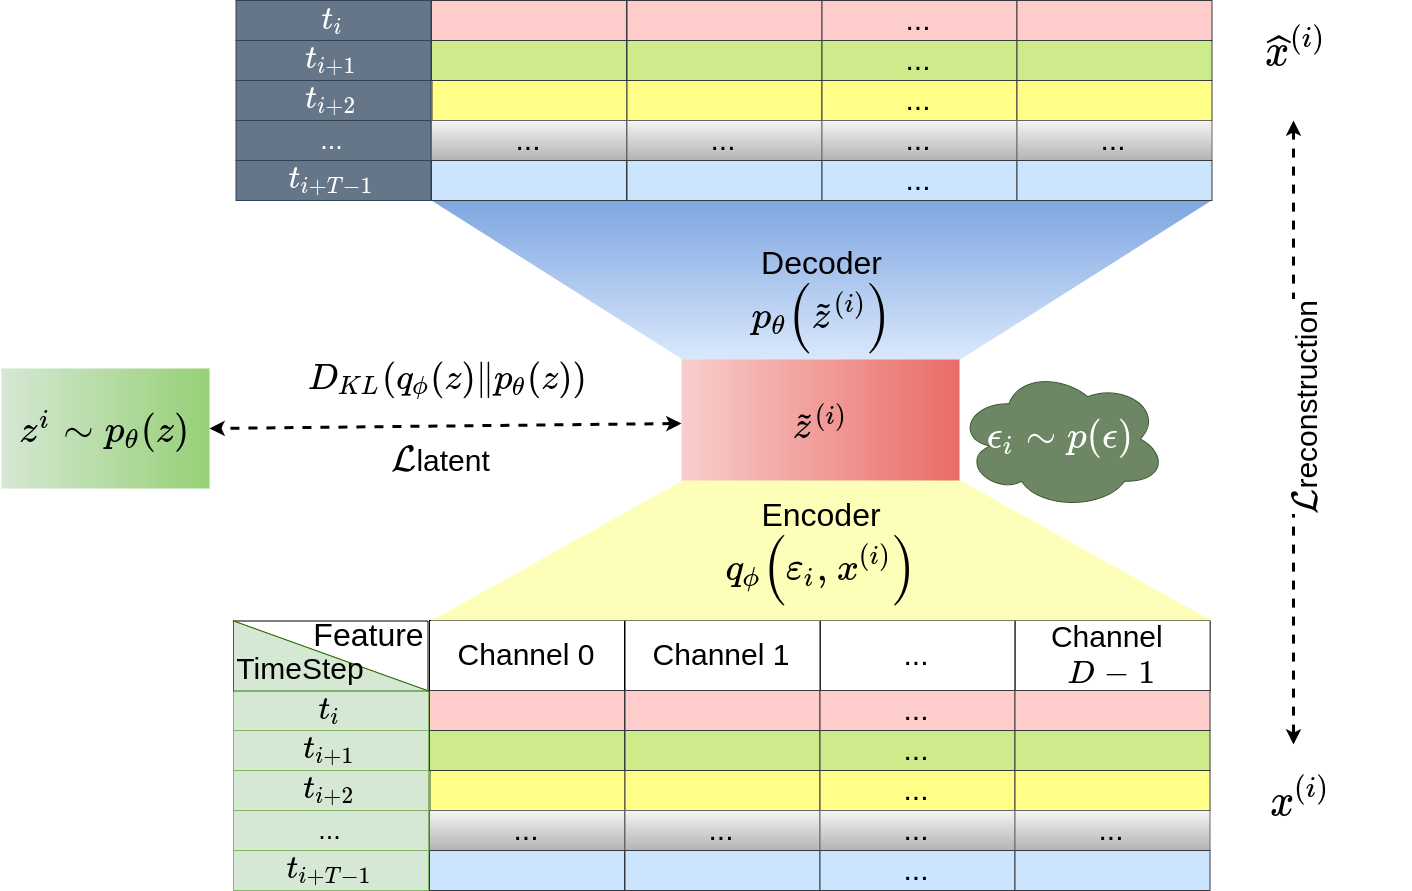
\includegraphics[width=1.0\textwidth]{figures/VAE/pngs/VAE_Arch.png}
	\caption{Kiến trúc mô hình dựa trên Variational Auto Encoder}
	\label{fig:VAE-arch}
\end{figure}

Để chi tiết hơn mô hình, chúng tôi sử dụng các kí hiệu cho các giả thiết sau:
\begin{itemize}
    \item $X = \{x^{(i)}\}_{i=1}^N$ gồm $N$ các điểm dữ liệu có phân phối đồng nhất độc lập (iid).
    \item Giá trị $z^{(i)}$ được sinh ra từ phân phối tiên nghiệm $p_{\theta^*}(z)$.
    \item Giá trị $x^{(i)}$ được sinh ra từ phân phối đồng thời $p_{\theta^*}(x \given z)$.
\end{itemize}

 Mục tiêu của bài toán là việc dự đoán cần phải chính xác đồng thời mô hình tìm được phân phối của dữ liệu đã cho theo phân phối tiên nghiệm. Trong phần thực nghiệm, chúng tôi có sử dụng mạng nơ-ron cho từng mô-đun vì lý do dễ dàng cập nhật trọng số  khi có được hàm lỗi.
 
 \textbf{Hàm lỗi cho việc phân loại:} $\mathcal{L}_C$ dựa được tính theo lỗi của hàm softmax.
 \textbf{Hàm lỗi cho việc tối đa likelihood theo phân phối tiên nghiệm:}
\begin{align}
  \mathcal{L}_{MLE} = -\frac{1}{N} \sum_{i=1}^N log(p_\theta(x^{(i)}))  
\end{align}

Với mô-đun Encoder, Decoder và Classifier là hàm tất định, tuy nhiên vì lý do $z$ được sinh mẫu ngẫu nhiên nên không thể xây dựng hàm lỗi một cách trực tiếp vì lý do khi khai triển $p_\theta(x)$:
\begin{equation} \label{eq:intractable_likelihood}
p_\theta(x) = \int p_\theta(z)p_\theta(x \given z) dz
\end{equation}
với :
\begin{itemize}
    \item $p_\theta(z)$ là phân phối tiên nghiệm có thể tính được.
    \item $p_\theta(x \given z)$ là phân phối có thể tính được thông qua mô-đun Decoder.
\end{itemize}

Tuy nhiên không thể tính được (intractable) cho toàn bộ $z$ trên miền liên tục. Khi khai triển phân phối hậu nghiệm: $p_\theta(z \given x)$ đưa về dạng không thể phân giải được do $p_\theta(x)$:
\begin{align}
  p_\theta(z \given x) = \frac{p_\theta(x \given z)p_\theta(z)}{p_\theta(x)}\label{eqn:intractable_posterior}.
\end{align}
Một cách giải quyết vấn đề trên là xấp xỉ hàm lỗi theo phương pháp suy luận biến phân được trình bày kĩ hơn tại Tiểu mục \ref{variational-lower-bound}. Theo phương pháp này khi khai triển $\log p_\theta(x)$:
\begin{align}
\log p_\theta(x^{(i)})  \geq \mathcal{L}(x^{(i)}, \theta, \phi) 
\end{align}
Với:

\begin{align}
\mathcal{L}(x^{(i)}, \theta, \phi) = \mathbb{E}_{z} \left[\log p_\theta(x^{(i)} \given z) \right]
    - \mathbb{E}_{z} \left[\log \frac{q_\phi(z \given x^{(i)})}{p_\theta(z)} \right]
\label{eq:elbo_loss}
\end{align}



Việc tối ưu $p_\theta(x^{(i)})$ thay bằng việc tối ưu cận dưới $\mathcal{L}(x^{(i)}, \theta, \phi)$. Lúc này hàm lỗi mới thay cho hàm $\mathcal{L}_{MLE}$ được tính như sau:
\begin{align}
  \mathcal{L}_{ELBO} &= -\frac{1}{N} \sum_{i=1}^N 
  \left(
  \mathbb{E}_{z} \left[\log p_\theta(x^{(i)} \given z) \right]
    - \mathbb{E}_{z} \left[\log \frac{q_\phi(z \given x^{(i)})}{p_\theta(z)} \right]
  \right)\\
  &= \mathcal{L}_{reconstruction} + \mathcal{L}_{latent}
\end{align}

Trở lại với kiến trúc VAE, phương trình  \eqref{eq:elbo_loss} 
có thể mô tả như sau:
\begin{itemize}
    \item $\mathbb{E}_{z} \left[\log p_\theta(x^{(i)} \given z) \right]$ : được tính theo mô-đun Decoder khi tái tạo lại $x$ từ $z$.
    \item $\Dkl{q_\phi(z \given x^{(i)})}{p_\theta(z)}$: Kullback–Leibler divergence giữa hai phân phối hậu nghiệm và tiên nghiệm.
\end{itemize}


\begin{subequations}\label{eq:sub}
	\noeqref{eq:1,eq:2}
	\begin{gather}
	\frac{\text{d}b_1}{\text{d}z} - \beta_1b_1 = C_{12}b_2,\label{eq:1}\\
	\frac{\text{d}b_2}{\text{d}z} - \beta_2b_2 = C_{21}b_1.\label{eq:2}
	\end{gather}
\end{subequations}
\eqref{eq:sub}


% Khi giá trị của hàm $\mathcal{L}_{ELBO}$ được giảm trong quá trình huấn luyện. Hai lỗi $$
Hai hàm lỗi được trực quan theo Hình \ref{fig:VAE-describe} dưới đây:
%%%%%%%%%%%%%%%%%%% Figure VAE loss describe
\begin{figure}[H]
	\center	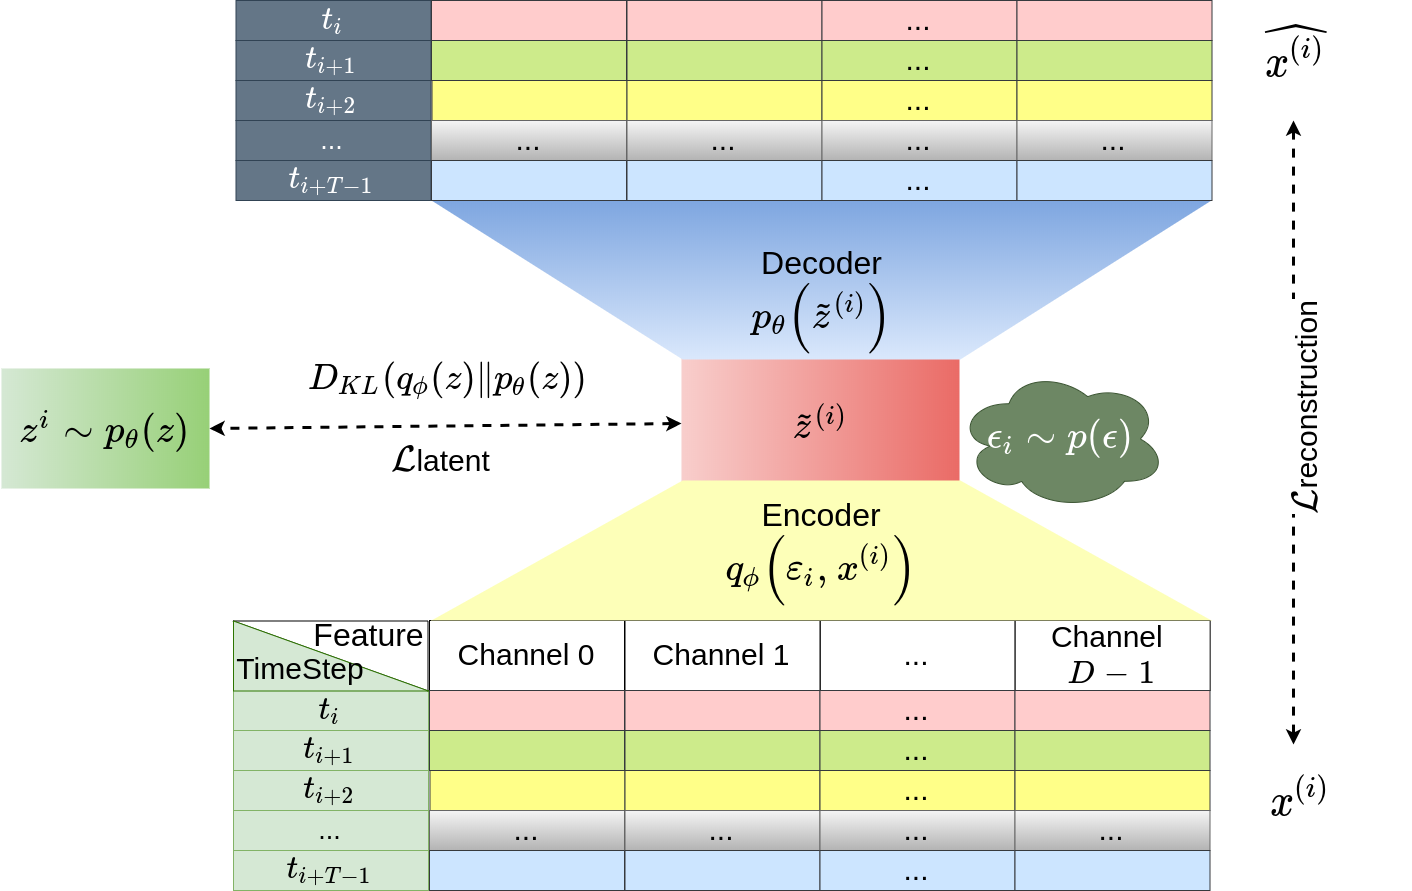
\includegraphics[width=1.0\textwidth]{figures/VAE/pngs/VAE_Arch_Describe.png}
	\caption{Mô tả hàm lỗi trong mô hình VAE}
	\label{fig:VAE-describe}
\end{figure}

Mục tiêu của bài toán là giảm được giá trị của hàm $\mathcal{L}_{ELBO}$. 
Trong trường hợp hội tụ cần đảm bảo phân phối hậu nghiệm $q_\phi(z \given x^{(i)})$ có các tham số từ mô-đun Encoder được tiến về phân phối tiên nghiệm cho trước: $p_\theta(z)$, đồng thời với phân phối hậu nghiệm có thể tái tạo lại dữ liệu cho trước. Nói cách khác, từ quá trình huấn luyện, mô hình có thể `học' được phân phối dữ liệu ban đầu từ phân phối tiên nghiệm đơn giản hơn được cho trước.

Trong phần hiện thực, chúng tôi có giả định biến ẩn (latent variable) có số chiều là $n_z$ thuộc phân phối multivariate normal distribution với vector trung bình là $\mu = 0 \in \mathbb{R}^{n_z}$, và hiệp phương sai là $\Sigma = I \in \mathbb{S}_{++}^{n_z}$. Theo đó, $ \mathcal{L}_{latent}$ được tính như sau:
\begin{align}
     \mathcal{L}_{latent} &= \Dkl{q_\phi(z \given x^{(i)})}{\mathcal{N}(0, I)}\\
     &= \frac{1}{2}\sum_{i=1}^{n_z}(\sigma_i^2 + \mu_i^2 - \log(\sigma_i^2) -1) \geq 0
\end{align}
Với dữ liệu thời gian, việc tính lỗi $\mathcal{L}_{reconstruction}$ không thể chuyển (scale) dữ liệu về khoảng $[0-1]$ vì trong phiên tiếp theo, các biến có giá trị vượt ngoài phạm vi $[0-1]$. Cụ thể, với 1 tháng trước tỷ giá trong phạm vi từ 2000 đến 5000, khi đưa dữ liệu tháng sau có tỷ giá là 5500 vượt ngoài khoảng trên. Vì lý do trên, chúng tôi lựa chọn hàm log mean square error để thể hiện lỗi khi tái tạo lại dữ liệu:
\begin{align}
     \mathcal{L}_{reconstruction} &= \frac{1}{N}\sum_{i=1}^N \log((x^{(i)} - \hat{x}^{(i)})^2) \geq 0
\end{align}

\begin{figure}[H]
	\center	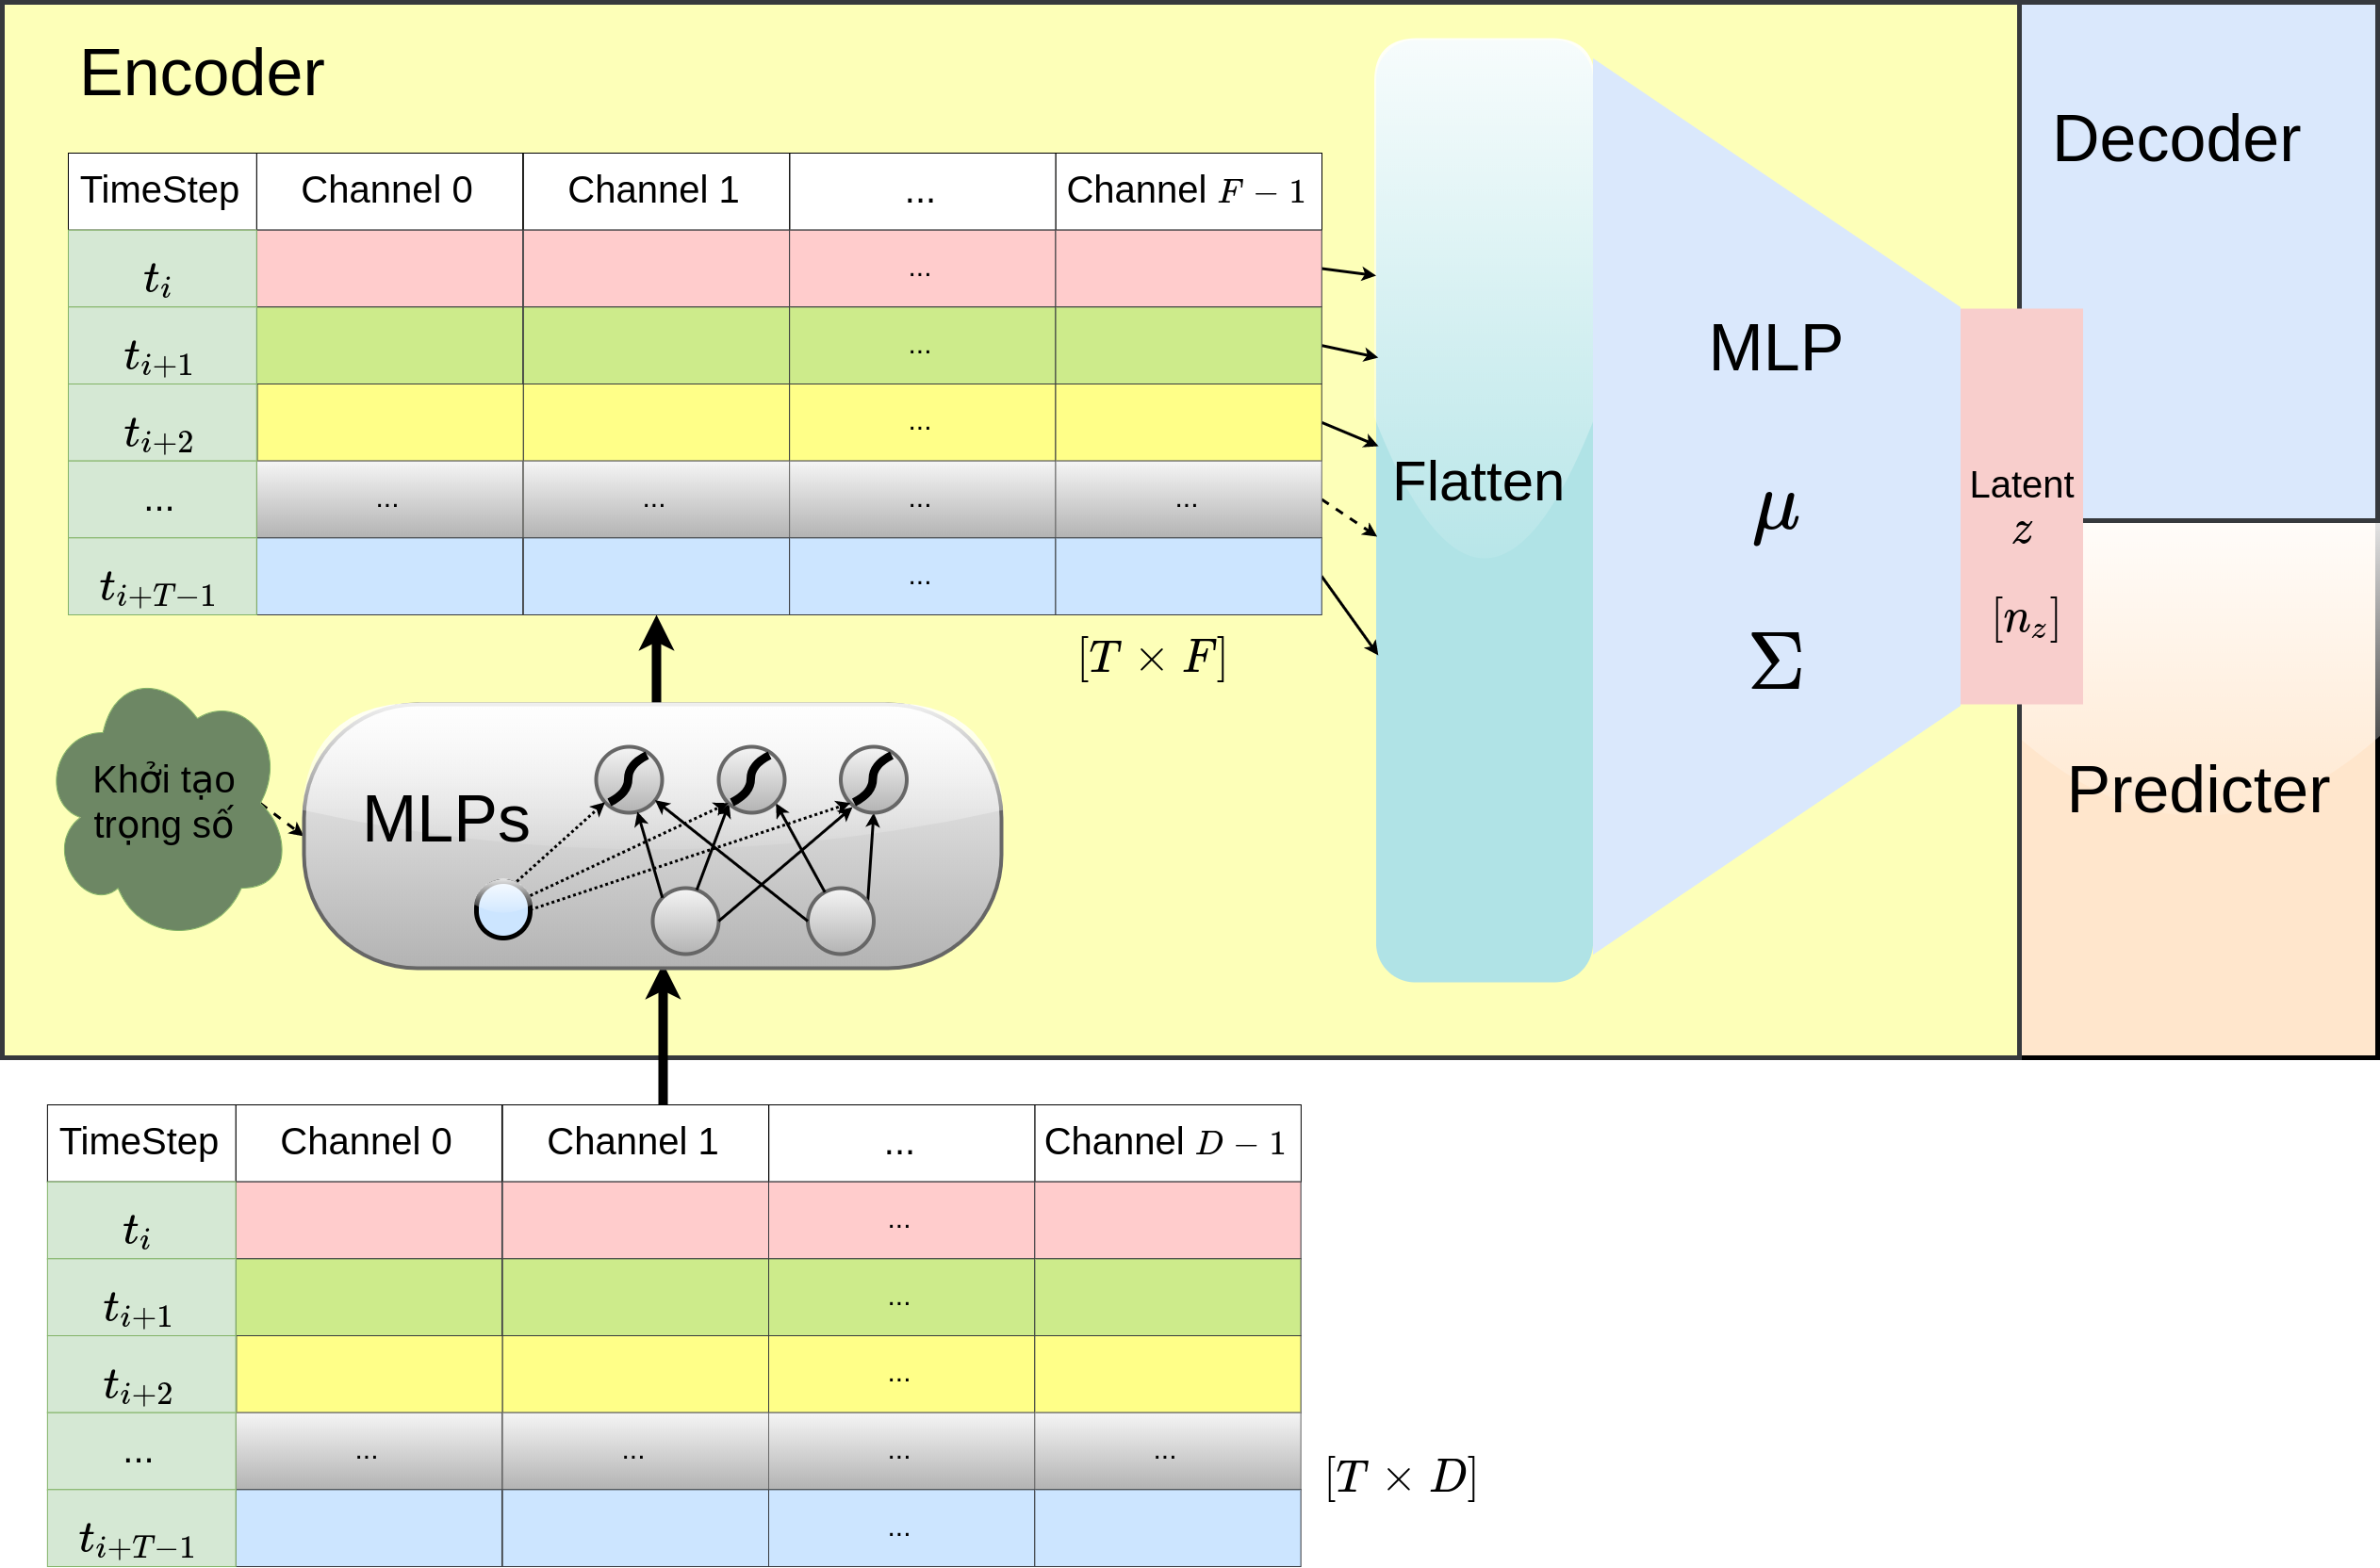
\includegraphics[width=1.0\textwidth]{figures/VAE/pngs/VAE_Encoder.png}
	\caption{Kiến trúc mô-đun Encoder}
	\label{fig:VAE-encoder}

\end{figure}

\chapter{Các khái niệm cơ bản có liên quan tới đề tài}

% Đại số tuyến tính linear algebra
% \input{chapters/concept_linear_algebra}
\section{Các khái niệm về tài chính}
\subsection{Tính thanh khoản (Liquidity)}
% https://www.binance.vision/economics/liquidity-explained

% Liquidity as a term is defined as the ability to buy or sell assets in the market without causing a drastic change in the assets price.
Khái niệm về tính thanh khoản dùng để chỉ mức độ mà một tài sản có thể được mua hoặc bán trên thị trường mà không làm ảnh hưởng nhiều đến giá thị trường.
% Liquidity can refer to two different areas; liquid market and liquid asset.
% Liquid market means that there are always investors in the market willing to trade. A liquid asset refers to an asset that can be easily converted into cash.
Khái niệm tính thanh khoản được chia thành 2 loại: tính thanh khoản thị trường (liquid market) và tính thanh khoản về tài sản (liquid asset). Thị trường có tính thanh khoản cao ám chỉ rằng trong thị trường thường xuyên có các nhà đầu tư sẵn sàng giao dịch. Một tài sản có tính thanh khoản cao đồng nghĩa với việc tài sản đó có thể chuyển đổi sang tiền mặt một cách dễ dàng. Đối với thị trường tiền mã hóa, để so sánh tính thanh khoản giữa các sàn trong cùng một thời điểm hoặc tính thanh khoản của một sàn tại những thời điểm khác nhau có 3 yếu tố quan trọng: 
%24 hour trading volume, Order book depth and the amount by which the ask price exceeds the bid price, also known as the bid/ask spread.
\begin{itemize}
	\item Lượng đồng giao dịch trong ngày.
	\item Số lượng lệnh mua/bán dựa trên danh sách lệnh (order book) được công khai dựa theo các sàn như Coinbase Pro\cite{live-order-book}, Binance, Bittrex, \dots
	\item Lượng chênh lệch giữa giá yêu cầu của bên bán và giá bỏ thầu của bên mua (bid/ask spread).
\end{itemize}

\subsection{Nhiễu (Noise)}
Khái niệm nhiễu có quan hệ đối lập với khái niệm thông tin (information) với dữ liệu giá cung cấp đầy đủ thông tin, việc dự đoán dễ dàng và ngược lại với dữ liệu có nhiễu cao do bị ảnh hưởng bởi các yếu tố khác như phần đề cập tại phần \ref{overview:factor}. Nhiễu khiến những quan sát của các nhà đầu tư không được hoàn hảo, điều này dẫn thị trường có khả lưu động\cite{noise-finance}.


%\section{Các khái niệm về xác suất}
\subsection{Hàm mật độ xác suất (Probability density function)}
Với các phiên giao dịch có các thành phần như giá mở, giá đóng, số lượng đồng giao dịch,\dots, ta có thể coi như các biến ngẫu nhiên liên tục tương ứng. Khái niệm hàm mật độ xác suất trong văn cảnh trên được hiểu như một hàm gồm các tham số thể hiện được mật độ phân bố của các biến ngẫu nhiên.
\begin{figure}[hbt!]
	\center	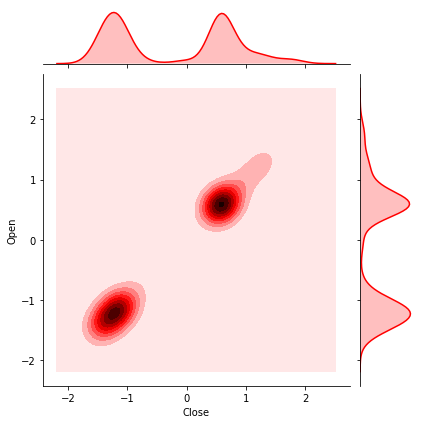
\includegraphics[width=0.8\textwidth]{probability/z_score_marginal_distribute_diff.png}
	\caption{Phân phối biên giá mở/đóng dữ liệu đã xử lý}
	\label{fig:z_score_marginal_distribution_diff}
\end{figure}
\FloatBarrier
Hình ~\ref{fig:z_score_marginal_distribution_diff} thể hiện mật độ của phân phối đồng thời giữa giá đóng và giá mở của các khối nến được biểu diễn dưới dạng $p_{data}(Open, Close)$.
\subsection{Hàm phân phối biên (Marginal distribution)}
Với dữ liệu liên tục như trên, hàm phân phối biên đối với giá mở được biểu diễn dưới dạng:
$p_{data}(Open) = \int_y p_{data}(Open, Close=y) dy = \int_y p_{data}(Open \given Close=y)p_{data}(Close=y)dy$ Một cách trực quan, hàm phân phối trên được biểu diễn bởi đường biên bên trái Hình ~\ref{fig:z_score_marginal_distribution_diff}

\subsection{Nhiễu trắng (White noise)}
Nhiễu trong dữ liệu như phần đề cập trong phần \ref{concept:finance:noise} có thể được giảm thiểu bằng cách tìm hàm phân phối của nhiễu bằng thống kê, nếu phân phối của nhiễu có dạng phân phối chuẩn với trung bình là 0, nhiễu này được gọi là nhiễu trắng Gauss (white Gaussian noise). Việc giảm thiểu nhiễu trong dữ liệu làm mô hình trở nên dễ tìm được mẫu đặc trưng (pattern) hơn.

\subsection{Biến ẩn (Latent variable)}
Biến ẩn được hiểu theo cách trừu tượng là biến không thể quan sát trực tiếp\cite[trang~264]{bishop} mà được suy luận từ biến quan sát được trong dữ liệu. Cụ thể hơn, với dữ liệu là giá của 100 ngày đầu một mô hình có khả năng tìm được quan hệ giữa giá ngày thứ 50 phụ thuộc nhiều vào giá ngày thứ 49 hơn so với ngày thứ 99, mô hình này được gọi là mô hình biến ẩn (latent variable model) với quan hệ được biểu diễn bằng phép toán có giá trị được lưu trong các biến ẩn.
\subsection{Mô hình đồ thị có hướng (Directed graphical model)}
Trong mô hình đồ thị có hướng hay mạng Bayes (Bayes network) việc suy diễn từ các trạng thái trước sang các trạng thái sau.
\begin{figure}[hbt!]
	\center	\includegraphics[width=0.6\textwidth]{Variational_inference/Bayes_inference.png}
	\caption{Mô hình mạng Bayes}
	\label{fig:Bayes_inference}
\end{figure}
Cụ thể với mô hình được được trực quan theo như Hình ~\ref{fig:Bayes_inference}, một giao dịch BTC/USD vào 6 giờ sáng ngày 31/7/2017 có giá mở là 2439.97\$, giá đóng là 2415.19\$, lượng giao dịch là 138.82 đồng BTC với xu hướng giao dịch tiếp theo có xác suất được kí hiệu là:
$P(Up \given Open =2727.26, Close=2740.01, Volume BTC = 385.41)$ với xác suất đồng thời của giao dịch và được tính:
%\begin{equation} \label{eq1}
%\begin{multline*}
\begin{equation}
\begin{split}
p(Up,Open = 2727.26, Close = 2740.01, Volume BTC = 385.41)\\
= p(Open = 2727.26) \cdot p(Close = 2740.01) \cdot p(Volume BTC = 385.41)\\
\cdot p(Pa(Up) \given Open =2727.26, Close=2740.01, Volume BTC = 385.41)\\
\cdot p(P_1 \given Open =2727.26, Close=2740.01, Volume BTC = 385.41)\\
\cdot p(Up \given Pa(Up), P_1)
\end{split}
\end{equation}



Một cách tổng quát xác suất đồng thời của giao dịch và xu hướng tăng giảm về giá của giao dịch tiếp theo được biểu diễn dưới dạng:
$p_\theta(x_1, x_2, \dots, x_M) = \prod_{i=1}^{M}p_\theta(x_j, Pa(x_j))$ với $Pa(x_j)$ giá trị của nút mạng trước đó (parent variable) của $x_j$.
\subsection{Suy luận biến phân (Variational inference)}
Phương pháp suy luận biến phân được sử dụng trong mô hình đồ thị có hướng\cite{intro_variational} với các biến ẩn $z$ và các quan sát $x$ với mục tiêu ước lượng được phân bố của $x$ được xấp xỉ bằng phân phối $Q(Z)$: $P(X \given Z) \approx Q(Z)$ với $Q(Z)$ là phân phối tiên nghiệm đơn giản hơn $P(Z|X)$.

Sử dụng độ đo bất đồng Kullback–Leibler nhằm thể hiện sự khác nhau giữa phân phối $Q$ so với phân phối $P$: 


$\Dkl{Q}{P} \triangleq  \mathbb{E}_{Q(Z)} [\log \frac{Q(Z)}{P(Z \given X)}]$

Sử dụng luật Bayes:
$\Dkl{P}{Q} = \mathbb{E}_{Q(Z)} [\log \frac{Q(z)}{P(z , x)}  + \log P(x)]$\\
hay:\\
$\log(P(x)) = \Dkl{P}{Q} - \mathbb{E}_{Q(z)} [\log \frac{Q(z)}{P(z , x)}]
= \Dkl{P}{Q} + \mathcal{L}(Q)
$


\section{Các khái niệm về mô hình sinh, mô hình phân biệt}
Khái niệm mô hình sinh và mô hình phân biệt ở đây được sử dụng trong ngữ cảnh học có giám sát.
\subsection{Mô hình sinh (Generative Model)}
Với dữ liệu đầu vào là $x$ được gán nhãn y trong quá trình tiền xử lý, mô hình sinh học được phân bố đồng thời của x và y $p_\theta(x,y)$ thông qua việc ước lượng các giá trị của các thông số trong $\theta$ việc suy diễn nhãn đối với dữ liệu kiểm thử được thực hiện bằng cách sử dụng luật Bayes\cite{gen-vs-dis} để tính $p_\theta(y\given x)$ sau đó tính giá trị dự đoán của nhãn với $\hat{y}$ có độ tin cậy cao nhất:
$\hat{y} = \argmax\limits_{y \in \mathcal{D}_y} p_\theta(y\given x)$. Với định nghĩa này một mô hình khi có đầu vào gồm các giao dịch và các thuộc tính được thêm vào từ bước xử lý dữ liệu mô hình có khả năng học được phân bố của các giao dịch và có thể sinh ra được các giao dịch mới theo phân bố tương tự như phân bố của dữ liệu được coi là mô hình sinh hay mô hình sinh mẫu.
%%%%%%%%%%%%%%%%%%%%%%%%%%%%%%%%%%%%%%%%%%%%%%%%%%%%%%%%%
\subsection{Mô hình phân biệt (Discriminative Model)}
Mô hình phân biệt học được phân bố $p_\theta(y \given x)$, việc suy diễn nhãn được tính trực tiếp từ dữ liệu kiểm thử. Với định nghĩa này một mô hình có cùng dữ liệu trên chứa thông tin của các giao dịch và đầu ra là xu hướng tăng hoặc giảm của giao dịch hoặc giá tiếp theo của giao dịch được gọi là mô hình phân biệt.
%%%%%%%%%%%%%%%%%%%%%%%%%%%%%%%%%%%%%%%%%%%%%%%%%%%%%%%%%



%\subsection{Likelihood}



\chapter{Thí nghiệm với mô hình}

\section{Phân tích hiện thực mô hình tham khảo}
\subsection{Xử lý dữ liệu bài toán}
Yêu cầu của bài toán là dự đoán giá của các đồng với nhau. Bài toán có thể chia ra làm 2 loại như sau:
\begin{itemize}
	\item Phân loại giá tăng hoặc giảm trong một khoảng thời gian kế tiếp.
	\item Dự đoán giá của các đồng xác định trong phạm vi liên tục tại thời gian kế tiếp.
\end{itemize}
Các mô hình đã tham khảo thuộc bài toán học có giám sát, dữ liệu được chia thành 3 ph

\subsection{Áp dụng dữ liệu vào mô hình rừng ngẫu nhiên}
 Đề tài có sử dụng thư viện hỗ trợ scikit-learn để xây dựng rừng ngẫu nhiên.
 Rừng ngẫu nhiên có đầu vào là dữ liệu ở dạng bảng với mỗi thuộc tính (mỗi cột) có thể ở dạng loại rời rạc (category) hoặc liên tục (numerical). Khi áp dụng dữ liệu thô, với mỗi quan sát là một dòng thuộc bảng và nhãn là giá lên hoặc xuống, đối với giá trong 1 phút sau ta có thể phân ra 2 loại tăng hoặc giảm. Tuy nhiên với mỗi quan sát trước có thể phụ thuộc vào nhiều quan sát trước đó, việc sử dụng các cây CART chỉ với một giao dịch là không phù hợp,ta có thể thêm các thuộc tính như giá trung bình trong 1 giờ trước đó, trong một ngày trước đó, \dots
 
 \subsection{Áp dụng dữ liệu vào mô hình mạng nơron tích chập}
 Đề tài có sử dụng thư viện hỗ trợ keras trên nền tensorflow một thư viện mã nguồn mở có hỗ trợ khả năng tính toán của các bộ xử lý đồ họa. Trong bước tiền xử lý dữ liệu để đưa vào trong mạng có sử dụng mỗi cửa sổ trượt làm một ảnh một chiều với số kênh là số thuộc tính của mỗi giao dịch, độ dài của mỗi ảnh được định nghĩa trước là số giao dịch liên tục. Nhãn của những ảnh này là xu hướng tăng hoặc giảm của giao dịch cuối cùng với mỗi ảnh.\\
 Khi dữ liệu được đưa vào mạng nơron cần được chuẩn hóa để tránh hiện tượng các nơron không cập nhật được khi hàm kích hoạt có họ ReLU hoặc khó kích hoạt khi các hàm kích hoạt phi tuyến khác như hàm sigmoid hoặc hàm tanh.\\ Các bước \textbf{chuẩn hóa dữ liệu} được mô tả như sau:
 \begin{itemize}
 	\item Các thuộc tính về thời gian đổi về dạng số nguyên theo chuẩn UNIX.Các số này khá lớn nên được chuẩn hóa dạng logarit, sau đó chuẩn hóa theo standard score.
 	%TODO Standard score viết công thức
 	\item Các thuộc tính còn lại như lượng giao dịch, giá mở, giá đóng theo dạng standard score
 \end{itemize}

Dữ liệu được đưa vào mạng nơron tích chập với ý tuởng chính như sau:


\begin{algorithm}[H]
	\KwData{507918 giao dịch bitcoin/Yên}
	\KwResult{Mô hình với các tham số, độ chính xác khi test}
	\textbf{Khởi tạo:}\\
	\begin{itemize}
		\item Chuẩn hóa dữ liệu theo từng cột.
		\item Tập train: 480000 bộ cửa sổ đầu, mỗi cửa sổ chứa 100 giao dịch liên tục nhau, mỗi cửa sổ liên tiếp nhau 1 giao dịch.
		\item Các tham số của mô hình tại mỗi lớp.
		\item $\ell=\infty$
	\end{itemize}
	\While{Khi số lượng bộ test nhỏ hơn 1024}{
		Tập test : sau 100 giao dịch tiếp theo so với tập train lấy 1024 bộ cửa sổ liên tiếp.\;
		Lấy tập test làm tập kiểm định;
		Tính $\ell$ là Loss của mô hình đối với tập kiểm định;

		\If{$\ell_1 < \ell$}{
			Cập nhật tham số\; $\ell = \ell_1$\;
		}
		Tập train: tăng kích thước của tập train thêm lên 1024 cửa sổ tiếp theo.
	}
	\caption{Áp dụng kĩ thuật rolling window}
\end{algorithm}

Khi áp dụng standard score, với mỗi thuộc tính có giá trị trung bình về 0 và phương sai về 1. Điều này ảnh hưởng tốt cho mạng nơron tích chập khi hội tụ nhanh và khó bị `kẹt lại' ở những điểm thung lũng hơn.

% \dots
 % TODO dụng dữ liệu thô như hình 1.1
 
 \section{Kết quả}
 Các số liệu kết quả trong phần này được lấy từ các lần thực nghiệm huấn luyện trên google colab, một nền tảng dịch vụ có hỗ trợ phần cứng và thư viện miễn phí, với dữ liệu đầu vào từ  2012-01-01 đến 2018-11-11 và độ chính xác theo bài toán phân loại lên hoặc xuống.
 
  \textbf{Mô hình rừng ngẫu nhiên} Kết quả cho độ chính xác là 53\%. \\
  \textbf{Mô hình mạng nơron tích chập} Kết quả cho độ chính xác là 71\% được tính bằng trung bình của 65 lần kiểm thử cuối. %Kết quả được mô tả như hình sau:\\
  %\includegraphics{figures/} 
 % TODO: get information about google clould resource
 
 

\chapter{Thí nghiệm và đánh giá} \label{chap-Implement}
Trong hai chương trước có đề cập tới các mô hình tham khảo và cách thu thập, xử lý dữ liệu để chuẩn bị cho quá trình thí nghiệm. Tiếp sau đây, trong chương này sẽ trình bày thư viện sử dụng, mô tả tham số trong mô hình. Dựa trên kết quả các mô hình từ đó rút ra các nhận xét về mô hình sử dụng và các điểm hạn chế khi hiện thực đồng thời đưa ra các hướng phát triển của luận văn.

\section{Các độ đo được sử dụng}
Trong phần này, chúng tôi trình bày các độ đo được sử dụng để đánh giá các mô hình. Trước
hết, chúng tôi trình bày ma trận nhầm lẫn (confusion matrix) cho các nhãn dự đoán như trong Bảng 
% \ref{tab:confusion_matrix} 
\narrowlinespacing

\begin{table}[H] 
    \centering

    \begin{tabularx}{0.9\textwidth}{
    p{\dimexpr.2\linewidth-2\tabcolsep-1.0\arrayrulewidth}% column 1
    p{\dimexpr.2\linewidth-2\tabcolsep-1.0\arrayrulewidth}% column 2
    p{\dimexpr.25\linewidth-2\tabcolsep-1.0\arrayrulewidth}
    p{\dimexpr.25\linewidth-2\tabcolsep-1.0\arrayrulewidth}
    }
        
        \toprule\midrule
        \textbf{} & \textbf{} & \multicolumn{2}{c}{\textbf{Kết quả dự đoán}} \\
        % \midrule
        \cmidrule(rl){3-4}
        \textbf{} & \textbf{} & \textbf{Giá tăng} & \textbf{Giá giảm} \\
        \midrule
        \multirow{2}{*}{\textbf{Nhãn thực tế }}  & \textbf{Giá tăng} & True Positive (TP) & 
        False Positive (FP)\\
        & \textbf{Giá giảm} & False Negative (FN) & True Negative (TN) \\
        % \hline
        \midrule
        \bottomrule
        
    \end{tabularx}
    \label{tab:confusion_matrix}
    \caption{Ma trận nhầm lẫn  cho các nhãn dữ liệu}
\end{table}

\normallinespacing


% \section{Thí nghiệm Rừng ngẫu nhiên}
% Trong quá trình huấn luyện, mô hình rừng ngẫu nhiên cho kết quả gần như tuyệt đối, tuy nhiên khi kiểm định trên các tháng cuối mô hình đạt khoảng 53-55\% với nhiều lần chạy. Với kết quả trên ngoài các độ đo như f1-score, độ chính xác, đề tài sử dụng cách kiểm định cross-validation nhằm xác định độ sai khác mẫu (pattern) giữa các phiên giao dịch. Kết quả 
%  \narrowlinespacing

\begin{table}[H] 
    \centering

    \begin{tabularx}{0.7\textwidth}{
    p{\dimexpr.2\linewidth-2\tabcolsep-1.0\arrayrulewidth}% column 1
    p{\dimexpr.2\linewidth-2\tabcolsep-1.0\arrayrulewidth}% column 2
    p{\dimexpr.15\linewidth-2\tabcolsep-1.0\arrayrulewidth}
    p{\dimexpr.15\linewidth-2\tabcolsep-1.0\arrayrulewidth}
    }
        
        \toprule\midrule
        \textbf{} & \textbf{} & \multicolumn{2}{c}{\textbf{Kết quả dự đoán}} \\
        % \midrule
        \cmidrule(rl){3-4}
        \textbf{} & \textbf{} & \textbf{Giá giảm} & \textbf{Giá tăng} \\
        \midrule
        % \hline
        
        %[[682 423]
        %   [393 662]] -> 0.6222222222222222
        
%         % 3 months
        % [[7592 5462]
        %  [4420 8446]] -> 0.61875
        \multirow{2}{*}{\textbf{Nhãn thực tế }}  & \textbf{Giá giảm} & 487 & 562\\
        & \textbf{Giá tăng} & 388 & 723 \\
        
        % [[487 562]
        %  [388 723]]
        % \hline
        \midrule
        \bottomrule
        
    \end{tabularx}
    \label{tab:rf_confusion_matrix}
    \caption{Ma trận nhầm lẫn từ mô hình rừng ngẫu nhiên}
\end{table}

\normallinespacing

%  Kết quả cho độ chính xác là 56.02\%. \\
 
% \section{Thí nghiệm mô hình Máy học véctơ hỗ trợ}

% \textbf{Mô hình SVM} Kết quả được tính bằng trung bình của 3 tháng cuối tương ứng với 2160 phiên liên tục. Kết quả được mô tả theo bảng dưới đây:\\

% % \narrowlinespacing

\begin{table}[H] 
    \centering

    \begin{tabularx}{0.7\textwidth}{
    p{\dimexpr.2\linewidth-2\tabcolsep-1.0\arrayrulewidth}% column 1
    p{\dimexpr.2\linewidth-2\tabcolsep-1.0\arrayrulewidth}% column 2
    p{\dimexpr.15\linewidth-2\tabcolsep-1.0\arrayrulewidth}
    p{\dimexpr.15\linewidth-2\tabcolsep-1.0\arrayrulewidth}
    }
        
        \toprule\midrule
        \textbf{} & \textbf{} & \multicolumn{2}{c}{\textbf{Kết quả dự đoán}} \\
        % \midrule
        \cmidrule(rl){3-4}
        \textbf{} & \textbf{} & \textbf{Giá giảm} & \textbf{Giá tăng} \\
        \midrule
        % \hline
        
        % [[555 494]
        %  [473 638]]
        
%         % 3 months
%         [[6700 6354]
%           [3840 9026]]
        \multirow{2}{*}{\textbf{Nhãn thực tế }}  & \textbf{Giá giảm} & 555 & 494\\
        & \textbf{Giá tăng} & 473 & 638 \\
        % \hline
        \midrule
        \bottomrule
        
    \end{tabularx}
    \label{tab:svm_confusion_matrix}
    \caption{Ma trận nhầm lẫn từ mô hình SVM}
\end{table}

\normallinespacing


% \narrowlinespacing

\begin{table}[H] 
    \centering

    \begin{tabularx}{0.7\textwidth}{
    p{\dimexpr.2\linewidth-2\tabcolsep-1.0\arrayrulewidth}% column 1
    p{\dimexpr.2\linewidth-2\tabcolsep-1.0\arrayrulewidth}% column 2
    p{\dimexpr.15\linewidth-2\tabcolsep-1.0\arrayrulewidth}
    p{\dimexpr.15\linewidth-2\tabcolsep-1.0\arrayrulewidth}
    }
        
        \toprule\midrule
        \textbf{} & \textbf{} & \multicolumn{2}{c}{\textbf{Kết quả dự đoán}} \\
        % \midrule
        \cmidrule(rl){3-4}
        \textbf{} & \textbf{} & \textbf{Giá giảm} & \textbf{Giá tăng} \\
        \midrule
        % \hline
        
        % [[555 494]
        %  [473 638]]
        
%         % 3 months
%         [[6700 6354]
%           [3840 9026]]
        \multirow{2}{*}{\textbf{Nhãn thực tế }}  & \textbf{Giá giảm} & 555 & 494\\
        & \textbf{Giá tăng} & 473 & 638 \\
        % \hline
        \midrule
        \bottomrule
        
    \end{tabularx}
    \label{tab:svm_confusion_matrix}
    \caption{Ma trận nhầm lẫn từ mô hình SVM}
\end{table}

\normallinespacing

    
% Kết quả trên đưa ra độ chính xác 55.23\%

% \section{Thí nghiệm mô hình Hồi quy Logistic}

%  \narrowlinespacing

\begin{table}[H] 
    \centering

    \begin{tabularx}{0.7\textwidth}{
    p{\dimexpr.2\linewidth-2\tabcolsep-1.0\arrayrulewidth}% column 1
    p{\dimexpr.2\linewidth-2\tabcolsep-1.0\arrayrulewidth}% column 2
    p{\dimexpr.15\linewidth-2\tabcolsep-1.0\arrayrulewidth}
    p{\dimexpr.15\linewidth-2\tabcolsep-1.0\arrayrulewidth}
    }
        
        \toprule\midrule
        \textbf{} & \textbf{} & \multicolumn{2}{c}{\textbf{Kết quả dự đoán}} \\
        % \midrule
        \cmidrule(rl){3-4}
        \textbf{} & \textbf{} & \textbf{Giá giảm} & \textbf{Giá tăng} \\
        \midrule
        % \hline
        
        % [[605 444]
        %  [508 603]] -> 0.5592592592592592
        
%         % 3 months
        % [[8069 4985]
        %  [4284 8582]] -> 0.6423996913580247
        \multirow{2}{*}{\textbf{Nhãn thực tế }}  & \textbf{Giá giảm} & 605 & 444\\
        & \textbf{Giá tăng} & 508 & 603 \\
        % \hline
        \midrule
        \bottomrule
        
    \end{tabularx}
    \label{tab:lr_confusion_matrix}
    \caption{Ma trận nhầm lẫn từ mô hình hồi quy logistic}
\end{table}

\normallinespacing

 
%  \textbf{Mô hình hồi quy logistic} Kết quả cho độ chính xác là 55.93\%.
 
% \section{Thí nghiệm mô hình dựa trên VAE}

% \narrowlinespacing

\begin{table}[H] 
    \centering
    \caption{Ma trận nhầm lẫn từ mô hình VAE}
    \begin{tabularx}{0.7\textwidth}{
    p{\dimexpr.20\linewidth-2\tabcolsep-1.0\arrayrulewidth}% column 1
    p{\dimexpr.20\linewidth-2\tabcolsep-1.0\arrayrulewidth}% column 2
    p{\dimexpr.15\linewidth-2\tabcolsep-1.0\arrayrulewidth}
    p{\dimexpr.15\linewidth-2\tabcolsep-1.0\arrayrulewidth}
    }
        
        \toprule\midrule
        \textbf{} & \textbf{} & \multicolumn{2}{c}{\textbf{Kết quả dự đoán}} \\
        % \midrule
        \cmidrule(rl){3-4}
        \textbf{} & \textbf{} & \textbf{Giá giảm} & \textbf{Giá tăng} \\
        \midrule
        % \hline
        
% [[566 481]
%  [496 617]] -> 0.5476851851851852


%         % 3 months
%         [[6700 6354]
%           [3840 9026]]
        \multirow{2}{*}{\textbf{Nhãn thực tế }}  & \textbf{Giá giảm} & 566 & 481\\
        & \textbf{Giá tăng} & 496 & 617 \\
        % \hline
        \midrule
        \bottomrule
        
    \end{tabularx}
    \label{tab:vae_confusion_matrix}
\end{table}

 
%  \textbf{Mô hình dựa trên VAE} Kết quả cho độ chính xác là 54.76\%.
%  \subsection{Áp dụng dữ liệu vào mô hình mạng nơron tích chập}
%  Đề tài có sử dụng thư viện hỗ trợ keras trên nền tensorflow một thư viện mã nguồn mở có hỗ trợ khả năng tính toán của các bộ xử lý đồ họa. Trong bước tiền xử lý dữ liệu để đưa vào trong mạng có sử dụng mỗi cửa sổ trượt làm một ảnh một chiều với số kênh là số thuộc tính của mỗi giao dịch, độ dài của mỗi ảnh được định nghĩa trước là số giao dịch liên tục. Nhãn của những ảnh này là xu hướng tăng hoặc giảm của giao dịch cuối cùng với mỗi ảnh.\\
%  Khi dữ liệu được đưa vào mạng nơron cần được chuẩn hóa để tránh hiện tượng các nơron không cập nhật được khi hàm kích hoạt có họ ReLU hoặc khó kích hoạt khi các hàm kích hoạt phi tuyến khác như hàm sigmoid hoặc hàm tanh.\\ Các bước \textbf{chuẩn hóa dữ liệu} được mô tả như sau:
%  \begin{itemize}
%  	\item Các thuộc tính về thời gian đổi về dạng số nguyên theo chuẩn UNIX.Các số này khá lớn nên được chuẩn hóa dạng logarit, sau đó chuẩn hóa theo standard score.
%  	%TODO Standard score viết công thức
%  	\item Các thuộc tính còn lại như lượng giao dịch, giá mở, giá đóng theo dạng standard score
%  \end{itemize}

% Dữ liệu được đưa vào mạng nơron tích chập với ý tuởng chính như sau:

\section{Kết quả}
\subsection{So sánh kết quả các mô hình đề xuất}

Chúng tôi so sánh kết quả dự đoán của bốn mô hình được sử dụng trong luận văn trên tập dữ liệu giao dịch từ ngày 2017/08/17 gồm hai khung thời gian phiên là 1 giờ và 5 phút cho ra các kết quả trong bảng:
\begin{table}[H] 
    \centering

    \begin{tabularx}{0.8\textwidth}
    {
    p{\dimexpr.4\linewidth-2\tabcolsep-1.0\arrayrulewidth}% column 1
    p{\dimexpr.2\linewidth-2\tabcolsep-1.0\arrayrulewidth}% column 2
    p{\dimexpr.2\linewidth-2\tabcolsep-1.0\arrayrulewidth}
    }
        
        \toprule
        \textbf{Mô hình} & \textbf{Độ chính xác} & \textbf{f1 score} \\
        % \cmidrule
        \midrule
        \textbf{Rừng ngẫu nhiên} & \textbf{rf} & \textbf{rf} \\
        \textbf{SVM} & \textbf{svm} & \textbf{svm} \\
        \textbf{Hồi quy Logistic} & \textbf{lr} & \textbf{lr} \\
        \textbf{VAE} & \textbf{vae} & \textbf{vae} \\
        \bottomrule
        
    \end{tabularx}
    \label{tab:1h_compare}
    \caption{Kết quả dự đoán trên 1 giờ (đơn vị: \%)}
\end{table}



\begin{table}[H] 
    \centering

    \begin{tabularx}{0.8\textwidth}
    {
    p{\dimexpr.4\linewidth-2\tabcolsep-1.0\arrayrulewidth}% column 1
    p{\dimexpr.2\linewidth-2\tabcolsep-1.0\arrayrulewidth}% column 2
    p{\dimexpr.2\linewidth-2\tabcolsep-1.0\arrayrulewidth}
    }
        
        \toprule
        \textbf{Mô hình} & \textbf{Độ chính xác} & \textbf{f1 score} \\
        % \cmidrule
        \midrule
        \textbf{Rừng ngẫu nhiên} & 61.88 & \textbf{rf} \\
        \textbf{SVM} & 60.67 & svm \\
        \textbf{Hồi quy Logistic} & 64.24 & \textbf{lr} \\
        \textbf{VAE} & \textbf{vae} & \textbf{vae} \\
        \bottomrule
        
    \end{tabularx}
    \label{tab:1h_compare}
    \caption{Kết quả dự đoán trên 5 phút (đơn vị: \%)}
\end{table}
% TODO: nhận xét




% : Rừng ngẫu nhiên, Máy học véctơ hỗ trợ, hồi quy logistic và mô hình dựa trên VAE




% \begin{algorithm}[H]
	\KwData{507918 giao dịch bitcoin/Yên}
	\KwResult{Mô hình với các tham số, độ chính xác khi test}
	\textbf{Khởi tạo:}\\
	\begin{itemize}
		\item Chuẩn hóa dữ liệu theo từng cột.
		\item Tập train: 480000 bộ cửa sổ đầu, mỗi cửa sổ chứa 100 giao dịch liên tục nhau, mỗi cửa sổ liên tiếp nhau 1 giao dịch.
		\item Các tham số của mô hình tại mỗi lớp.
		\item $\ell=\infty$
	\end{itemize}
	\While{Khi số lượng bộ test nhỏ hơn 1024}{
		Tập test : sau 100 giao dịch tiếp theo so với tập train lấy 1024 bộ cửa sổ liên tiếp.\;
		Lấy tập test làm tập kiểm định;
		Tính $\ell$ là Loss của mô hình đối với tập kiểm định;

		\If{$\ell_1 < \ell$}{
			Cập nhật tham số\; $\ell = \ell_1$\;
		}
		Tập train: tăng kích thước của tập train thêm lên 1024 cửa sổ tiếp theo.
	}
	\caption{Áp dụng kĩ thuật rolling window}
\end{algorithm}

% Khi áp dụng standard score, với mỗi thuộc tính có giá trị trung bình về 0 và phương sai về 1. Điều này ảnh hưởng tốt cho mạng nơron tích chập khi hội tụ nhanh và khó bị `kẹt lại' ở những điểm thung lũng hơn.

% % \dots
%  % TODO dụng dữ liệu thô như hình 1.1
%   \subsection{Áp dụng dữ liệu vào mô hình mạng Long Short-term Memory}
%  Mô hình mạng LSTM có ưu điểm 
%  Các số liệu kết quả trong phần này được lấy từ các lần thực nghiệm huấn luyện trên google colab, một nền tảng dịch vụ có hỗ trợ phần cứng và thư viện miễn phí, với dữ liệu đầu vào từ  xxxxxxxxx và độ chính xác theo bài toán phân loại lên hoặc xuống.
 
 

 

  
  %\includegraphics{figures/} 
 % TODO: get information about google clould resource


% Appendix A

\chapter*{Phụ lục} % Main appendix title
% Frequently Asked Questions
\subsection{Một số thuật ngữ được sử dụng}
\textbf{Block}: là một cấu trúc dữ liệu chứa dữ liệu của giao dịch.

\textbf{Blockchain}: một cuốn sổ cái công khai chứa thông tin của các giao dịch đã được thực hiện trên hệ thống. Nó bao gồm một chuỗi các block theo trình tự thời gian. Các block bao gồm các giao dịch và thông tin từ các khối trước đó. Một đường dẫn duy nhất từ block đầu tiên đến khối hiện tại được sử dụng và mỗi block sẽ bao gồm mã băm của block trước đó.

\textbf{Mining}: bước xác thực cần phải có cho mỗi giao dịch tiền mã hóa và để thêm các bản ghi vào Blockchain.

\textbf{Mã băm}: một hàm một chiều lấy dữ liệu đầu vào có kích thước bất kỳ và tạo ra kết quả có độ dài cố định. Việc tính toán mã băm phải nhanh và dễ dàng, việc đảo ngược mã phải khó và tốn nhiều thời gian, chi phí đồng thời phải tránh tối đa đầu vào khác nhau cho ra kết quả giống nhau (tránh đụng độ).

\textbf{Peer-to-peer}: kiểu thiết kế hệ thống kết nối trực tiếp người dùng với người dùng mà không
thông qua một hệ thống quản lý trung gian nào. Đây là một hệ thống có kiến trúc phân tán.

\textbf{Public key và Private key}: là một cách mã hóa sử dụng một cặp khóa. Mỗi người dùng có một cặp mã khóa Public key và Private key này. Public key là khóa công khai mà mọi người ai cũng đều biết đến, xem như một cách để mọi người xác định một người cụ thể nào đó. Private key là khóa bí mật, chỉ chủ sở hữu mới biết mã bí mật của mình và không được tiết lộ cho người khác. Cơ chế hoạt động của cách mã hóa này là giao dịch sẽ được gửi và mã hóa với khóa công khai của người nhận. Chỉ người nhận có khóa bí mật tương ứng với khóa công khai này có thể giải mã được giao dịch trên.

\textbf{Double-spending}: lỗi phát sinh khi thực hiện các giao dịch bằng hệ thống điện tử. Lỗi này xuất hiện khi một khoản tiền được dùng để chi tiêu cho hai hay nhiều việc cùng lúc, khi đó hệ thống chưa giải quyết xong giao dịch trước, chưa trừ đi số tiền giao dịch thì đã
phát sinh giao dịch sau.

\section{Những yếu tố tác động đến giá trị đồng tiền mã hóa} \label{overview:factor}
\subsection{Cung, cầu và nhiễu trong thị trường}\label{overview:market-noise}
Trong nguyên tắc chính của kinh tế nếu nhu cầu mua đối với một đồng tiền tăng, giá trị của đồng tiền sẽ tăng và ngược lại khi nhu cầu bán tăng, giá sẽ giảm. Cụ thể khi thị trường tuân theo một quy luật chung (pattern) giá 3 ngày của cặp đồng A/B liên tục tăng và đến ngày thứ tư giảm theo chu kì. Khi một nhà đầu tư H phát hiện được tính chất này, đến ngày thứ tư trong chu kì sẽ thực hiện bán đồng A để kiếm lợi khiến giá thị trường bị điều chỉnh lại và có xu hướng tăng tại ngày thứ tư, nói cách khác thị trường sẽ thay đổi quy luật (pattern) trên bởi lệnh bán của người H, hay lệnh bán này gây ra nhiễu cho thị trường đồng A/B.
\subsection{Tin tức trên các phương tiện thông tin đại chúng}
Các sự kiện chính trị và kinh tế trên toàn thế giới ảnh hưởng đến cách mà con người phản ứng với các dự đoán giá, tin tức cảnh báo về rủi ro tác động chính lên cung-cầu.
\subsection{Quy định của chính phủ}
Có 4 cấp độ quản lý tiền ảo hiện nay đang được các nước áp dụng, cụ thể như sau:
\begin{itemize}
	% \item Cấm trên diện rộng.
	
	\item Cấm trên diện rộng:
	\item Cấm trong lĩnh vực tài chính ngân hàng (trong đó có Trung Quốc, Nga).
	% \item Cảnh báo rủi ro đối với người sử dụng, đầu tư.
	% \item  Chấp nhận như một phương tiện thanh toán (các nước chấp nhận đồng bitcoin gồm có Mỹ, Canada, Úc, Liên minh châu Âu, Phần Lan \cite{CountriesAllowBTC} ).
	
	
\end{itemize}
\subsection{Chính sách của các tổ chức}
Facebook, Google và Twitter đã ngăn chặn khách hàng và người dùng sử dụng dịch vụ cryptocurrency.
\subsection{Các vấn đề kỹ thuật}
Khi đồng tiền mật mã bị khai thác bằng các lỗ hổng từ Rủi ro khi sử dụng đồng tiền mã hóa 
Khi tài khoản mã hóa bị tấn công bằng kĩ thuật 

\subsection{Tính thanh khoản}
% https://www.binance.vision/economics/liquidity-explained

% Liquidity as a term is defined as the ability to buy or sell assets in the market without causing a drastic change in the assets price.
Khái niệm về tính thanh khoản (Liquidity) dùng để chỉ mức độ mà một tài sản có thể được mua hoặc bán trên thị trường mà không làm ảnh hưởng nhiều đến giá thị trường.
% Liquidity can refer to two different areas; liquid market and liquid asset.
% Liquid market means that there are always investors in the market willing to trade. A liquid asset refers to an asset that can be easily converted into cash.
Khái niệm tính thanh khoản được chia thành 2 loại: tính thanh khoản thị trường (liquid market) và tính thanh khoản về tài sản (liquid asset). Thị trường có tính thanh khoản cao đồng nghĩa với việc trong thị trường thường xuyên có các nhà đầu tư sẵn sàng giao dịch. Một tài sản có tính thanh khoản cao mang nghĩa rằng tài sản đó có thể chuyển đổi sang tiền mặt một cách dễ dàng. Đối với thị trường tiền mã hóa, để so sánh tính thanh khoản giữa các sàn trong cùng một thời điểm hoặc tính thanh khoản của một sàn tại những thời điểm khác nhau có 3 yếu tố quan trọng: 
%24 hour trading volume, Order book depth and the amount by which the ask price exceeds the bid price, also known as the bid/ask spread.
\begin{itemize}
	\item Lượng đồng giao dịch trong ngày.
	\item Số lượng lệnh mua/bán dựa trên danh sách lệnh (order book) được công khai dựa theo các sàn như Coinbase Pro, Binance, Bittrex \footnote{\url{https://www.cryptometer.io/data/coinbase_pro/btc/usd} truy cập vào ngày 2019/04/18}, \dots
	\item Lượng chênh lệch giữa giá yêu cầu của bên bán và giá đặt của bên mua (bid/ask spread).
\end{itemize}

\section{Nhu cầu sử dụng tiền mã hoá của mỗi hệ sinh thái}
\begin{itemize}
	\item Số thành viên tham gia vào hệ sinh thái (Số người đến khu vui chơi mua vé tham gia các trò chơi trong đó bằng tiền A).
	\item Số lượng dịch vụ trong hệ sinh thái (Khu vui chơi có càng nhiều trò chơi thì nhu cầu sử dụng tiền A càng tăng); Và các nền tảng như Ethereum luôn mở cho các đối tác tạo các dịch vụ gia tăng trên đó giống như khu vui chơi cho phép đối tác bên ngoài vào tổ chức trò chơi ở trong.
	\item  Số người đầu cơ: Những người nhận thấy nhu cầu tiền mã hoá của một hệ sinh thái tăng dần sẽ mua để nắm giữ chờ tăng giá thì bán ra. (Giống như phe vé bóng đá ngày trước mua vé chờ sát trận nhu cầu tăng vọt thì bán ra. Khu vui chơi thì ít có nhóm này vì lượng vé không bị giới hạn).
	\item  Số người bán bên ngoài chấp nhận tiền mã hoá: Một số người bán nhận thấy tính thanh khoản của tiền mã hoá và giá trị tăng dần của nó nên đã chấp nhận khách hàng thanh toán các hàng hoá dịch vụ của mình bằng loại tiền này (Nhà hàng bên cạnh khu vui chơi có thể chấp nhận khách hàng thanh toán bằng tiền A).
\end{itemize}

Thị trường luôn bị biến động do ảnh hưởng của các yếu tố. Trong chương này, chúng tôi sẽ đề cập tới những yếu tố cơ bản tác động lên đồng tiền mã hóa. Tiếp theo sau đó chúng tôi sẽ trình bày các chiến lược kèm theo ưu, nhược điểm khi trao đổi ngắn hạn trên đồng mã hóa.


\section{Giao dịch tiền mã hóa}
Các sàn tiền mã hóa cung cấp các lệnh giao dịch cơ bản: mua, bán với những cặp đồng (pair) với nhau, ngoài ra còn có thêm phương thức mua, bán tiền ảo bằng tiền mặt thông qua sàn đóng vai trò như bên thứ ba.\par
Để đảm bảo các đồng mã hóa có giá trị, cần một đồng có giá trị ổn định (stable coin) có giá trị cố định, với 1 USDT có giá trị ngang với 1 USD. Một đồng ổn định kể trên cần có những hai tính chất: Đáng tin cậy (có một tập đoàn có tài sản tương ứng đứng ra đảm bảo số đồng không bị lạm phát) và không bị thao túng (có giải thuật để kiểm soát số lượng đồng dựa trên tài sản thế chấp hoặc các đồng tiền mã hóa có liên quan). Các đồng ổn định hiện nay gồm:
TrueUSD (TUSD), USD Tether (USDT), USD Coin (USDC), Digix Gold Tokens (DGX), trong đó đồng USDT có tổng giá trị lưu thông đạt tới 4.4 tỉ USD\footnote{\url{https://stablecoinindex.com} truy cập vào ngày 2019/10/17}, cao nhất trong các đồng ổn định.

Các mô hình và chiến lược trong luận văn được đánh giá dựa trên tổng giá trị của các đồng mã hóa tại một thời điểm được quy về USDT.

\section{Các chiến lược giao dịch ngắn hạn}\label{strategy_describing}
Hai chiến lược cơ bản được nghiên cứu và thực hiện trong đề tài như sau:
\begin{itemize}
	\item Giao dịch cùng một loại cặp với nhau tại hai thời điểm khác nhau nhằm tăng số lượng đồng ban đầu.
	\item Giao dịch nhiều cặp với nhau theo một vòng dựa theo giá tại cùng một thời điểm.
	Hai chiến lược trên sẽ được trình bày chi tiết hơn trong phần tiếp theo. Tiếp sau đó, phần \ref{risk-strategy} sẽ trình bày rủi ro và tiềm năng của thị trường, từ đó làm nỗi bật các hạn chế, ưu điểm của từng chiến lược tương ứng.
\end{itemize}
Với dữ liệu được lấy từ sàn, có thể tạo một đánh giá thị trường với giao dịch ngắn hạn có tiềm năng hay không? Từ đó có thể tạo ra công cụ với khả năng dự đoán để tự động giao dịch không?  Nhằm trả lời cho hai câu hỏi trên, trong chương này sẽ đề cập tới hai phần chính:
\begin{itemize}
	\item Các chiến lược cơ bản được đề ra và mô phỏng hai chiến lược trên dữ liệu đã có. Ứng dụng các mô hình học máy để dự đoán xu hướng giá.
	\item  Đánh giá rủi ro của hai chiến lược thông qua giá có trước, từ đó nhận định tiềm năng của thị trường.
\end{itemize}
\subsection{Chiến lược giao dịch cùng một loại cặp đồng}\label{describe_strategy_1}
Khi giao dịch cùng một loại cặp đồng A/B theo thời gian khác nhau, đặt lệnh mua hay đổi đồng B để mua A khi tỷ giá A/B có xu hướng giảm ngược lại đặt lệnh bán khi tỷ giá có xu hướng tăng. Chiến lược này sẽ không hiệu quả khi giá ở mỗi phiên không chênh lệch nhau nhiều đặc biệt có trường hợp lỗ khi mỗi lần giao dịch sễ mất tiền phí do bên sàn thu. Vì vậy chiến lược nói trên sẽ được thêm một ràng buộc là  ngưỡng phí giao dịch $\epsilon$ và các biến:
\begin{itemize}
	\item $W^a_t$: số đồng A quy ra B theo giá tại thời điểm $t$.
	\item $W^b_t$: số đồng B quy ra A theo giá tại thời điểm $t$.
	\item $y_t$: tỷ giá đồng A/B tại thời điểm $t$.
	\item $a$, $b$: số đồng A, số đồng B trong ví tại thời điểm đang xét.
\end{itemize}
Với $t$ là thời điểm gần nhất giao dịch, xét tại thời điểm $\tau$ xảy ra sau đó, Việc đặt lệnh mua phải thỏa yêu cầu sau:
$W^a_\tau > W^a_t$ hay:
\begin{align}
\frac{b}{y_\tau}(1-\epsilon) > \frac{b}{y_t}   
\end{align}
do đó: $y_\tau < y_t(1 -\epsilon)$  \\
Tương tự, việc đặt lệnh bán phải thỏa yêu cầu sau:
$W^b_\tau > W^b_t$ hay:
\begin{align}
a (1 - \epsilon) y_\tau > ay   
\end{align}



hay $y_\tau(1 -\epsilon) > y_t $

Việc mô phỏng chiến lược này cần tuân theo ràng buộc của sàn như sau: đơn vị tối thiểu là 0.000001 BTC và 0.01 USDT ví dụ muốn mua cặp đồng trên khi có 1.234 USDT với số lượng tối đa phí giao dịch sẽ là 0.1\% với giá khớp lệnh là 8000 số lượng USDT còn lại trong ví là 0.004 số lượng giao dịch sẽ là 1.23 USDT, số lượng BTC nhận vào ví là $1.23/8000*(1-0.1/100) = 0.00015359625$.



\subsection{Chiến lược giao dịch nhiều loại cặp đồng}
Với 3 đồng là A, B, C, việc chuyển đồng A chuyển sang đồng B, chuyển đồng B sang đồng C và cuối cùng chuyển lại đồng C sang đồng A tạo thành một vòng lặp, việc đồng A tăng lên hoặc giảm đi có thể xảy ra. Trong cùng một phiên giao dịch, việc tìm vòng lặp như trên sao cho số lượng đồng A được tăng lên so với trước đòi hỏi các lần chuyển đổi giữa các cặp diễn ra liên tục và có thứ tự nói cách khác tất cả các lần giao dịch đều phải được hoàn thành, đây cũng là nhược điểm của chiến lược này vì trong khi biết giá của các giao dịch trước, giá của các cặp sẽ đổi khi thực hiện giao dịch đòi hỏi giao dịch phải diễn ra nhanh.
Lấy ví dụ ở thời điểm lúc 8 giờ ngày 04/01/2018 xét 3 cặp đồng là BTC/USDT, ETH/BTC, ETH/USDT có tỉ giá tương ứng là 15172.12, 0.060893, 920.08 với phí giao dịch cho mỗi lần trao đổi mặc định là 0.1\% đối với sàn Binance, với 1.0 USDT lần lượt đổi các cặp là USDT sang ETH, ETH sang BTC và BTC sang USDT số đồng USDT thu về trong ví là 1.0011 với giả thiết ở mỗi giao dịch đều đổi hết (bỏ qua ràng buộc về số đồng tối thiểu). Trong ví dụ này với 3 đồng trên ta có thể thấy một cách trực quan rằng số đồng USDT tăng sau một vòng chuyển đổi. Việc tìm các vòng chuyển đổi tại mỗi thời điểm như trên có thể  được mô hình hóa bằng bài toán như sau:
\begin{algorithm}[H]
	\KwData{$T$ phiên giao dịch; $\frac{N(N-1)}{2}$ cặp tương ứng với $N$ đồng}
	\KwResult{Số lần xuất hiện vòng có xu hướng làm tăng số lượng đồng ban đầu}
	\textbf{Khởi tạo:}\\
	
	\begin{itemize}
		\item Đồ thị hai phía đầy đủ.
		\item Tensor $M$ kích thước $TxNxN$ chứa thông số của $T$ phiên giao dịch.
		\item Phí giao dịch $\epsilon$.
		\item $t = 0$.
	\end{itemize}
	\For{t trong T}{
		Cập nhật trọng số của đồ thị\\
		Khi không có giao dịch giữa hai đồng A/B trọng số cạnh $d(A,B) \gets 1e-20$;
		$d(B,A) \gets 1e-20$\\
		
		\For{u, v trong $M_t$}{
			$d(u,v) \gets -log(d(u,v)) - log(\epsilon))$ \Comment{Chuyển sang giá trị logarit}
		}
	
		
		\If{Đồ thị có trọng số âm}{
			% $t.insert(1)$
			$t \gets t + 1$\\
			Tìm chu trình nhỏ nhất không lặp.
		}
	}	
	\caption{Tìm số lượng phiên giao dịch có thể  làm tăng số đồng ban đầu.}
\end{algorithm}
Thống kê với phí giao dịch mặc định là 0.1\% đối với sàn Binance từ 2018-01-01 đến 2019-09-21 gồm 15000 phiên giao dịch với khoảng thời gian mỗi phiên là 1 giờ xét trên 3 đồng BTC, ETH, USDT được thu thập từ 3 cặp: USDT/ETH, ETH/BTC, BTC/USDT đưa ra 75 lần đồ thị tồn tại chu trình âm. Khi thêm đồng BNB đồ thị với 4 loại đồng gồm 6 cặp, con số này đạt 1027 lần.
% TODO: notebook tăng eps, tăng số đồng -> tạo bảng

\section{Rủi ro và tiềm năng của thị trường}\label{risk-strategy}
\subsection{Chiến lược giao dịch trên một cặp đồng}
Khi thực hiện khảo sát chiến lược trao đổi trên một cặp, với dữ liệu thu được trên sàn Binance với cặp đồng BTC/USDT trong khoảng thời gian từ 2017-08-17
đến 2019-09-01, giả sử số tiền trong ví ban đầu là 1.0 BTC các ngưỡng phí  $\epsilon$ được thay đổi cho ra kết quả được thống kê trong bảng sau:

\definecolor{Gray}{gray}{0.9}
\definecolor{LightCyan}{rgb}{0.88,1,1}
\definecolor{maroon}{cmyk}{0,0.87,0.68,0.32}

\begin{table}[ht]
	
	\centering % used for centering table
	\begin{tabular}{c c c c c} % centered columns (4 columns)
		\hline\hline %inserts double horizontal lines
		% Thời gian bắt đầu & Ngưỡng phí (\%) & Số lần giao dịch & Tổng USDT đầu & Tổng USDT sau \\ [0.5ex] % /home/nam/Dropbox/thesis/src/strategy_POC/notebook/.ipynb_checkpoints/Strategy_01-POC-report-checkpoint.ipynb
		\multirow{2}{*}{Thời gian bắt đầu}  & \multirow{2}{*}{Ngưỡng phí (\%)} &
		\multirow{2}{*}{Số lần giao dịch} & 
		\multirow{2}{*}{Tổng USDT đầu} & 
		\multirow{2}{*}{Tổng USDT sau} \\[2.5ex] %
		\hline % inserts single horizontal line
		\rowcolor{maroon!10}
		2017/08/28 13:00:00 & 0.1 & 129 & 4221.04 & 2193.22 \\
		% 2017-08-28 13:00:00 & 0.1 & 129 & 4221.04 & 2193.22 \\
		% inserting body of the table
		\rowcolor{maroon!10}
		2017/08/28 13:00:00 & 0.2 & 129 & 4221.04 & 2290.84 \\
		\rowcolor{LightCyan}
		2017/08/28 13:00:00 & 5 & 17 & 4221.04 & 6632.89 \\
		\rowcolor{LightCyan}
		2017/08/28 13:00:00 & 10 & 7 & 4221.04 & 6133.60 \\
		\rowcolor{maroon!10}
		2017/12/11 01:00:00 & 0.1 & 80 & 14975.03 & 9721.09 \\
		\rowcolor{maroon!10}
		2017/12/11 01:00:00 & 0.2 & 82 & 14975.03 & 9884.65 \\
		\rowcolor{LightCyan}
		2017/12/11 01:00:00 & 5 & 22 & 14975.03 & 17373.62 \\
		\rowcolor{maroon!10}
		2017/12/11 01:00:00 & 10 & 6 & 14975.03 & 13452.00 \\[1ex] % [1ex] adds vertical space
		
		% 2017-08-28 13:00:00 & 0.12 & 139 & 4221.04 & 2007.70 \\ [1ex] % [1ex] adds vertical space
		
		
		\hline %inserts single line
	\end{tabular}
	\label{table:nonlin} % is used to refer this table in the text
	
	\caption{Mô phỏng chiến lược giao dịch một cặp đồng theo thời gian}
\end{table}

% http://localhost:8888/notebooks/notebook/Strategy_01-POC-report.ipynb 
% Trade log -> Timestamp ->
Hạn chế dễ thấy của chiến lược này là không biết trước giá của phiên giao dịch tiếp theo. Cụ thể với ngày 2017/12/15 giá đạt ngưỡng cao nhất khi đó theo chiến lược, đổi hết đồng BTC sang thành USDT, tiếp theo giá giảm đều và qua ngưỡng phí và tiếp tục giảm, khi này số đồng USDT đã được chuyển sang BTC số lượng đồng BTC so với thời điểm trước khi bán ban đầu là nhiều hơn, khi giá tiếp tục giảm lệnh mua sẽ không được thực hiện do đã hết đồng USDT phải chờ đến khi giá tăng so với lần mua tại ngày 2018/16/03. Điều này dẫn tới việc tính theo giá USDT tổng giá trị BTC là giảm từ 14975.03 USDT xuống 13452 USDT. Để giảm rủi ro này, ta có thể dự đoán xu hướng giá đóng của phiên giao dịch kế tiếp
% tức vào ngày giá cao nhất TODO
, nếu giá có xu hướng giảm, lệnh mua sẽ được giữ lại tới khi giá có xu hướng tăng. Đây chính là ý tưởng chính cho việc hình thành bài toán dự đoán xu hướng giá ngắn hạn, các mô hình sẽ được học từ các phiên giao dịch trước và dự đoán xu hướng giá của phiên giao dịch sau. Việc đánh nhãn cho dữ liệu sẽ được trình bày trong phần \ref{data-labeling}.
% TODO tạo bảng 
\subsection{Chiến lược giao dịch trên nhiều cặp đồng}
Với chiến lược đổi trên nhiều đồng, khi tăng số lượng đồng, việc giao dịch theo chiến lược này trở lên khó khăn hơn vì khi duyệt chu trình, tất cả các cạnh đều phải đi qua, nói cách khác các lần đổi đều phải hoàn thành. Tuy nhiên trong quá trình đổi, giá của hai đồng sẽ không giữ nguyên như giá hiện tại, việc khớp giá sẽ khó xảy ra. Do đó, việc đặt lệnh các đồng nên được hiện thực cùng lúc. Ngoài ra, bổ sung mô hình dự đoán xu hướng giá của phiên giao dịch tiếp theo có thể hỗ trợ thêm cho chiến lược này để tính khả năng đồ có chu trình âm có thể được duyệt tại phiên sau.
% TODO histogram trên notebook

% TODO
%   số lần chạy| Thời gian bắt đầu| Tỷ lệ dự đoán |profit  min | profit max | avg profit

%   Trong Tiểu mục \ref{describe_strategy_1} khi giao dịch trên một cặp đồng, mức độ rủi ro và tiềm năng của chiến lược này phụ thuộc vào các yếu tố như thị trường và ngưỡng phí cho trước, lệnh giao dịch được đưa ra dựa trên giá hiện tại, bổ sung cho chiến lược này khi biết chính xác xu hướng giá cần và

% Với giao dịch trên nhiều đồng các thông số
% TODO
%   số lần chạy| Thời gian bắt đầu| Số sau 3 giao dịch |Số sau 5 giao dịch| Số giao dịch tiếp theo trung bình

% \end{itemize}
\addcontentsline{toc}{chapter}{Phụ lục A}
%\chapter{Cơ sở lý thuyết}
%\thispagestyle{empty}\newpage
%\chapter{Tổng quan về lĩnh vực nghiên cứu} 
\section{Những yếu tố tác động đến giá trị đồng tiền mã hóa} \label{overview:factor}
\subsection{Cung và cầu của thị trường}
Trong nguyên tắc chính của kinh tế nếu nhu cầu mua đối với một đồng tiền tăng, giá trị của đồng tiền sẽ tăng và ngược lại khi nhu cầu bán tăng, giá sẽ giảm.
\subsection{Tin tức trên các phương tiện thông tin đại chúng}
Các sự kiện chính trị và kinh tế trên toàn thế giới ảnh hưởng đến cách mà con người phản ứng với các dự đoán giá, tin tức cảnh báo về rủi ro tác động chính lên cung-cầu.
\subsection{Quy định của chính phủ}
Có 4 cấp độ quản lý tiền ảo hiện nay đang được các nước thực thi, cụ thể:
\begin{itemize}
\item Cấm trên diện rộng.
\item Cấm trong lĩnh vực tài chính ngân hàng (trong đó có Trung Quốc, Nga).
\item Cảnh báo rủi ro đối với người sử dụng, đầu tư.
\item  Chấp nhận như một phương tiện thanh toán (các nước chấp nhận đồng bitcoin gồm có Mỹ, Canada, Úc, Liên minh châu Âu, Phần Lan \cite{CountriesAllowBTC} ).
\end{itemize}
\subsection{Chính sách của các tổ chức}
Facebook, Google và Twitter đã ngăn chặn khách hàng và người dùng sử dụng dịch vụ cryptocurrency.
\subsection{Các vấn đề kỹ thuật}
Vì đồng tiền mã hóa có thể bị hack thành công vào tài khoản hoặc tấn công máy chủ, có thể làm giảm tỷ giá hối đoái, dẫn đến giá giảm.
\section{Nhu cầu sử dụng tiền mã hoá của mỗi hệ sinh thái}
\begin{itemize}
    \item Số thành viên tham gia vào hệ sinh thái (Số người đến khu vui chơi mua vé tham gia các trò chơi trong đó bằng tiền A).
    \item Số lượng dịch vụ trong hệ sinh thái (Khu vui chơi có càng nhiều trò chơi thì nhu cầu sử dụng tiền A càng tăng); Và các nền tảng như Ethereum luôn mở cho các đối tác tạo các dịch vụ gia tăng trên đó giống như khu vui chơi cho phép đối tác bên ngoài vào tổ chức trò chơi ở trong.
    \item  Số người đầu cơ: Những người nhận thấy nhu cầu tiền mã hoá của một hệ sinh thái tăng dần sẽ mua để nắm giữ chờ tăng giá thì bán ra. (Giống như phe vé bóng đá ngày trước mua vé chờ sát trận nhu cầu tăng vọt thì bán ra. Khu vui chơi thì ít có nhóm này vì lượng vé không bị giới hạn).
    \item  Số người bán bên ngoài chấp nhận tiền mã hoá: Một số người bán nhận thấy tính thanh khoản của tiền mã hoá và giá trị tăng dần của nó nên đã chấp nhận khách hàng thanh toán các hàng hoá dịch vụ của mình bằng loại tiền này (Nhà hàng bên cạnh khu vui chơi có thể chấp nhận khách hàng thanh toán bằng tiền A).
\end{itemize}
%\input {chapters/theory/deeplearning}
%\input {chapters/theory/data_training}
% \input {chapters/theory/type_labeling}

%\chapter{Các công trình liên quan}
%\thispagestyle{empty}\newpage
%\input {chapters/related_works/related_works}
%\input {chapters/related_works/vgg}
%\input {chapters/related_works/ssd}

%\chapter{Phương pháp sử dụng}
%\thispagestyle{empty}\newpage
%\input {chapters/proposal_solutions/prior_research_gvlab}
%\input {chapters/proposal_solutions/proposal_method}

%\chapter{Hệ thống hỗ trợ làm nhãn thông minh cho bài toán học sâu}
%\thispagestyle{empty}\newpage
%\input {chapters/system/require_analysis}
%\input {chapters/system/technology_selected}
%\input {chapters/system/system_architecture}
%\input {chapters/system/system_using}
%\input {chapters/system/deploy_system}

%\chapter{Tổng kết}
%\thispagestyle{empty}\newpage
%\input {chapters/summary/review}
%\input {chapters/summary/futurework}
%\input {chapters/summary/progress}

%\chapter{Tài liệu tham khảo}
\thispagestyle{empty}\newpage
\bibliographystyle{IEEEtran}
%\bibliography{reference}
\bibliography{myref}

\end{document}